%%
%% Toolbox Test Automation  Manual
%% PGL 2007
%%%%%%%%%%%%%%%%%%%%%%%%%%%%%%%%%%%%%%%%
% PDF compatibility code. 

\makeatletter
\newif\ifpdflatex@
\ifx\pdftexversion\@undefined
\pdflatex@false
%\message{Not using pdf}
\else
\pdflatex@true
%\message{Using pdf}
\fi

\newcommand{\latexpdf}[2]{
  \ifpdflatex@ #1
  \else #2
  \fi
}

\newcommand{\latexorpdf}[2]{
  \ifpdflatex@ #2
  \else #1
  \fi
}

\makeatother

\newcommand{\RuleTarget}[1]{\hypertarget{rule:#1}{}}
\newcommand{\Ruledef}[2]
{
  \RuleTarget{#1}\Rule{#1}{#2}%
  }
\newcommand{\Ruleref}[1]{
  \hyperlink{rule:#1}{#1}}


%%%%%%%%%%%%%%%%%%%%%%%%%%%%%%%%%%%%%%%%
\newcommand{\pformat}{a4paper}

\latexorpdf{
\documentclass[\pformat,12pt]{article}
}{
% pdftex option is used by graphic[sx],hyperref,toolbox.sty
\documentclass[\pformat,pdftex,12pt]{article}
}

\usepackage[dvipdfmx]{graphicx, color}

% definition of VDM++, JavaCC, JJTree, JTB, ANTLR and SableCC for listings
\usepackage{listings}
\setcounter{topnumber}{3}
\def\topfraction{1.0}
\setcounter{bottomnumber}{3}
\def\bottomfraction{1.0}
\setcounter{totalnumber}{3}
\def\textfraction{.1}
\renewcommand{\floatpagefraction}{0.8}
\usepackage{times}
\usepackage{color}
\lstdefinelanguage{VDM++}
  {morekeywords={\#act, \#active, \#fin, \#req, \#waiting, abs, all, allsuper, always, and, answer, 
     assumption, async, atomic, be, bool, by, card, cases, char, class, comp, compose, conc, cycles,
     dcl, def, del, dinter, div, do, dom, dunion, duration, effect, elems, else, elseif, end,
     error, errs, exists, exists1, exit, ext, floor, for, forall, from, functions, 
     general, hd, if, in, inds, infer, init, inmap, input, instance, int, inter, inv, inverse, iota, is, 
     isofbaseclass, isofclass, inv, inverse, lambda, let, map, mu, mutex, mod, nat, nat1, new, merge, 
     munion, not, of, operations, or, others, per, periodic, post, power, pre, pref, 
     private, protected, public, qsync, rd, responsibility, return, reverse, samebaseclass, 
     sameclass, psubset, rem, rng, sel, self, seq, seq1, set, skip, specified, st, 
     start, startlist, static, subclass, subset, subtrace, sync, synonym, then, thread, 
     threadid, time, tixe, tl, to, token, trap, types, undefined, union, using, values, 
     variables, while, with, wr, yet, RESULT, false, true, nil, periodic pref, rat, real},
   %keywordsprefix=mk\_,
   %keywordsprefix=a\_,
   %keywordsprefix=t\_,
   %keywordsprefix=w\_,
   sensitive,
   morecomment=[l]--,
   morestring=[b]",
   morestring=[b]',
  }[keywords,comments,strings]
\lstdefinelanguage{JavaCC}
  {morekeywords={options, PARSER\_BEGIN, PARSER\_END, SKIP, TOKEN},
   sensitive=false,
  }[keywords]

% define the layout for listings
\lstdefinestyle{tool}{basicstyle=\ttfamily,
                         frame=trBL, 
			 showstringspaces=false, 
			 frameround=ffff, 
			 framexleftmargin=0mm, 
			 framexrightmargin=0mm}
\lstdefinestyle{mystyle}{basicstyle=\ttfamily,
                         frame=trBL, 
%                         numbers=left, 
%			 gobble=0, 
			 showstringspaces=false, 
%			 linewidth=\textwidth, 
			 frameround=fttt, 
			 aboveskip=5mm,
			 belowskip=5mm,
			 framexleftmargin=0mm, 
			 framexrightmargin=0mm}
%\lstdefinestyle{mystyle}{basicstyle=\sffamily\small,
%			 frame=tb,
%                         numbers=left,
%			 gobble=0,
%			 showstringspaces=false,
%			 linewidth=345pt,
%			 frameround=ffff,
%			 framexleftmargin=8mm,
%			 framexrightmargin=8mm,
%			 framextopmargin=1mm,
%			 framexbottommargin=1mm,
%			 aboveskip=7mm,
%			 belowskip=5mm,
%			 xleftmargin=10mm,}

\lstset{style=mystyle}
\lstset{language=VDM++}
%\lstset{alsolanguage=Java}
% The command below enables you to escape into normal LaTeX mode inside your 
% VDM chunks by starting with a `!� character and ending with a `��
\lstset{escapeinside=!�}


\usepackage{toolbox}
\usepackage{vdmsl-2e}
\usepackage{makeidx}
\usepackage{alltt}
%\usepackage{epsfig}
\usepackage{here}
\usepackage{array}
\usepackage{longtable}
\usepackage{ifthen}
% plainpages=false: avoid warning
%   destination with the same identifier already exists
%   but it do not seem to work a the first pages
\latexorpdf{
\usepackage[dvipdfm,bookmarks=true,bookmarksnumbered=true,colorlinks,plainpages=true]{hyperref}
%\usepackage[plainpages=true,colorlinks,linkcolor=black,citecolor=black,pagecolor=black, urlcolor=black]{hyperref}
}{
\usepackage[plainpages=true,colorlinks]{hyperref}
}

\usepackage{vpp}

\newcommand{\Index}[1]{#1\index{#1}}

%\usepackage{latexsym}
%\usepackage{epsf}
% ueki
%\newcommand{\vpp}{\small\tt}
\renewcommand{\vpp}{\small\tt}
% ueki
\newcommand{\tr}[1]{{\bf\underline{#1}}}



\newcommand{\insertfig}[4]{ % Filename, epsheight, epswidth, caption,  label
\begin{figure}[H]
\begin{center}
\includegraphics[width=#2]{#1} 
\end{center}
\caption{{\em #3}} #4
\end{figure}
}

\newcommand{\insertfignw}[3]{ % Filename, caption,  label
\begin{figure}[h]
\begin{center}
\includegraphics{#1} 
\end{center}
\caption{{\em #2}} #3
\end{figure}
}

\newcommand{\insertfignwrot}[3]{ % Filename, caption,  label
\begin{figure}[h]
\begin{center}
\scalebox{1}%
{\rotatebox{270}{%
\includegraphics{#1}}}
\end{center}
\caption{{\em #2}} #3
\end{figure}
}

\makeindex


\newcommand{\vdmtoolsver}{V9.0.6}

\newcommand{\MYEQUIV}{$\equiv$}
\newlength{\nonstandlen}
\newcommand{\nonstandard}[1]{%
}
\newenvironment{TypeSemantics}{\begin{longtable}[r]{|p{3.5cm}|p{9cm}|}\hline%
  Operator Name & Semantics Description \\ \hline\hline \endhead}% 
  {\hline\end{longtable}}
  
%\renewcommand{\vdmpp}{{\small VDM}$^{++}$}

\makeatletter
% ------------- TOC manipulation ------------
\def\docglbldepth{1}
%\setcounter{secnumdepth}{\docglbldepth}
%\setcounter{tocdepth}{\docglbldepth}
\def\@pnumwidth{3.0em}
% more space for for >10 subsections
%\def\l@section{\@dottedtocline{1}{1.5em}{3.1em}}
\def\l@subsection{\@dottedtocline{2}{1.5em}{2.8em}}
%\def\l@subsubsection{\@dottedtocline{3}{4.3em}{3.6em}}
%\def\l@paragraph{\@dottedtocline{4}{7.9em}{4.1em}}
%\def\l@subparagraph{\@dottedtocline{5}{10em}{5em}}
\makeatother

\makeindex
%\latexpdf{\pdfinfo{
% /Title (The  VDM-SL Language)
% /Author (The VDM Tool Group, The Institute of Applied Computer Science)
%}}{}


\begin{document}
%\latexpdf{\pdfcatalog{/PageMode /UseOutlines} openaction goto page 1 {/Fit}}{}

\vdmtoolsmanualcsk{VDM++ Test Automation: VDMTesK}
        {\vdmtoolsver}
        {2016}
        {VDM++}
        {1.0}

\newcommand{\Lit}[1]{`{\tt #1}\Quote}
\newcommand{\Rule}[2]{
  \begin{quote}\begin{tabbing}
    #1\index{#1}\ \ \= = \ \ \= #2  ; %    Adds production rule to index
    
  \end{tabbing}\end{quote}
  }
\newcommand{\SeqPt}[1]{\{\ #1\ \}}
\newcommand{\lfeed}{\\ \> \>}
\newcommand{\dsepl}{\ $|$\ }
\newcommand{\dsep}{\\ \> $|$ \>}
\newcommand{\Lop}[1]{`{\sf #1}\Quote}
\newcommand{\blankline}{\vspace{\baselineskip}}
\newcommand{\Brack}[1]{(\ #1\ )}
\newcommand{\nmk}{\footnotemark}
\newcommand{\ntext}[1]{\footnotetext{{\bf Note: } #1}}
\newlength{\kwlen}
\newcommand{\Keyw}[1]{\settowidth{\kwlen}{\tt #1}\makebox[\kwlen][l]{\sf
    #1}}
\newcommand{\keyw}[1]{{\sf #1}}
\newcommand{\id}[1]{{\tt #1}}
\newcommand{\metaiv}[1]{\begin{alltt}\input{#1}\end{alltt}}

\newcommand{\OptPt}[1]{[\ #1\ ]}
\newcommand{\MAP}[2]{\kw{map }#1\kw{ to }#2}
\newcommand{\INMAP}[2]{\kw{inmap }#1\kw{ to }#2}
\newcommand{\SEQ}[1]{\kw{seq of }#1}
\newcommand{\NSEQ}[1]{\kw{seq1 of }#1}
\newcommand{\SET}[1]{\kw{set of }#1}
\newcommand{\PROD}[2]{#1 * #2}
\newcommand{\TO}[2]{$#1 \To #2$}
\newcommand{\FUN}[2]{#1 \To #2}
\newcommand{\PUBLIC}{\ifthenelse{\boolean{VDMpp}}{public\mbox{}}{\mbox{}}}
\newcommand{\PRIVATE}{\ifthenelse{\boolean{VDMpp}}{private}{\mbox{}}}
\newcommand{\PROTECTED}{\ifthenelse{\boolean{VDMpp}}{protected}{\mbox{}}}


% No line numbering
%\nolinenumbering
%\setindent{outer}{\parindent}
%\setindent{inner}{0.0em}


\section{Introduction}

Testing is one of the necessary stages of the software development
life cycle. It is applied at both the development and the maintenance
stages. Testing appears especially important during the development
and maintenance of critical software. In fact, only testing can
demonstrate to the developers and customers that a software program
does what is required, and does it as expected.

The size and the complexity of a test suite that provides a required
test completeness is comparable with the size of the program under
test, or even exceeds it. That is the reason why manufacturers often
have to economize on testing, which, in turn, typically increases the
cost of the maintenance stage.

To reduce the cost of testing during industrial software development to
an acceptable value, it is necessary to organize industrial test
development. In this case, the following are essential:

\begin{enumerate}
\item Elaborate a test suite architecture, i.e.\ to define a collection of
  test suite artifacts and relations between them.  
\item Evolve invariant components, which are identical for different
  test suites.  
\item For the specific components that depend on the target system,
  define ways of their generation based on compact and clear formal
  descriptions, and maximally increase reuse of such descriptions.  
\end{enumerate}

%On the basis of more than ten years experience in development of
%test suites for the industrial software and researches in employment
%of the program formal specifications \cite{Petrenko01}, we'd created
%the general methodology of test suites development, and also several
%projections of such methodology that are oriented onto concrete
%programming languages. In particular, the proposed VDM++TesK
%methodology is such a projection.

The VDM++TesK tool is an add-on feature that extends features of the
VDM++ version of VDMTools. VDM++TesK provides the developer of VDM++
models with new features enabling automation of parts of test suite
design and development, that allow to essentially increase the quality
of the models and, thus, to contribute to increase reliability
and other quality characteristics of the target software.

In the initial phase of getting acquainted with this feature, most
users may be confused with certain technical solutions that may be
uncommon. A number of basic concepts and constructs needed to master
to obtain the full benefits from this technology.
%Note, that to those who
%competent in VDM (and VDM++), it's easier to do it, because some
%unusual constructs (e.g. pre- and postconditions and invariants) are
%known to them. As regards to 
Complexity of the methodology, the following points should be kept in
mind:

\begin{itemize}
\item VDM++TesK had been developed for constructing test suites for
  large and critical software.  
\item 
%The main task of VDM++TesK is not debugging, when a rapid but
%  possibly cursory analysis of the robustness is often
%  needed. 
  VDM++TesK is mostly aimed at the industrial process of
  systematic testing, where the essential tasks are: evaluation of the
  test suite completeness, reuse of all testing process artifacts,
  etc.  
\item 
% VDM++TesK introduces additional features into the IFAD process
%  of real-time systems development. 
  The concepts of the VDM++TesK process is primarily
  based on the idea of a model's sequential complication. VDM++TesK
  potentially provides full support for this process. While
  solving problems of testing of models at each level and consistency
  of such levels, it is possible to achieve a high degree of test suite
  components reuse. It is also important for industrial projects that
  the test suite development and debugging activity can be started
  simultaneously with the prototype design and implementation.  
\end{itemize}

VDM++TesK is an implementation of the UniTesK concept of software
testing \cite{Bourdonov&02}. UniTesK is based on the experience of
deployment of the advanced industrial testing technologies. The
UniTesK concept has already been approved in companies such as Nortel
Networks, Microsoft Research and Intel. In these projects, the target
software was an operating system kernel and utilities,
telecommunication protocol implementations and various components of
compilers. UniTesK assumes that it is possible to implement its
concepts using different languages (and on multilanguage)
platforms. Several implementations already exist now (e.g.\ for
extended dialects of Java and C). VDM++TesK is such an implementation
for the VDM++ VDMTools platform.

First of all, the UniTesK concept proposes a novel view on the test
production using generation as much as possible. The underlying idea
is that it is not a test itself that is generated because this is
unmanageble for the most real-life systems, but instead a framework
for test suite is generated. This framework consists of three kinds of
components. The first kind is the pre-built components that are common
for all test suites of a certain kind. The second kind is the
components that are generated automatically. Sources for such
generation are pre- and postconditions and class invariants. The third
kind is so-called handmade components of a test suite. Usually, the
handmade components are operations of 2-3 lines in length, which
interfaces and purposes are defined by the UniTesK test suite
architecture. Notice, that a volume of handmade components in a test
suite usually does not exceed 5-10\%\ of the total amount.

%Difficulty of the UniTesK methodology acquirement is caused by its
%multicomponent architecture. Notice, that for users of OO libraries
%such as STL, the idea of UniTesK doesn't appear too novel. Here, like
%in real life, it will have to bear with just another demonstration of
%the conservation laws -- to save effort on test development, it's
%needed to spend an extra effort on the UniTesK concept acquirement. 

The current version of VDM++TesK is the first one that is offered to
VDM++ users. It has several limitations in comparison with other
implementations of UniTesK. At first, in regards to the fact that both
specification and executable model (that is the system under test) are
related to the same level of abstraction. In general case, UniTesK
allows data structures and even interfaces of a specification and an
implementation to differ (they are related to different abstraction
levels). The second limitation is the only criterion of the test
coverage completeness. Both of these limitations are not fundamental
and can be removed in future updates. 

%What's next? As it was mentioned above, use of this tool is preceded
%with the "initiation" to its ideology. If its doctrines would appear
%too sophisticated, have a look at "Specifications development" section
%or to the specification and test suite example. You will be convinced
%that separate steps of the test development technology are trivial. If
%it seems to you that you already can develop your specification and
%tests -- try to do it. If it seems to you that some components of
%test suite can be omitted -- just omit them, since UniTesK is
%intended to the very general case. If you fail, don't be despaired and
%come back to the UniTesK/VDM++TesK architecture description. 

\fbox{Reading guide for document}

\textbf{Terminological note.} Below, the term "model" will be used often. For
the VDM users, a model is a prototype written in VDM++. But in
UniTesK/VDM++TesK, the following conventions are accepted:

\begin{itemize}
\item A model is a kind of presentation of the target system's
  functionality/behavior (e.g. specifications in the form of pre- and
  postconditions, or a finite state machine that establishes the
  correlation between stimuli and reactions of the target
  system). Often (but not always), a model is more abstract and simple
  than its implementation.  
\item Terms ``implementation'', ``target system'', ``system under test'' are
  synonyms in this document, all these terms denote usual VDM++
  classes with explicit definition of their operations.  
\end{itemize}

\section{General VDM++TesK test suite architecture}

The VDM++TesK test suite is built according to the UniTesK concept
\cite{Bourdonov&02}. We begin describing its architecture with the
description of the UniTesK test suite.

\subsection{Terminology and General Principles}

UniTesK/VDM++TesK follows the "Design-by-contract" concept. First of
all, testing is aimed at verification of the correspondence between
the real behavior of an explicit VDM++ model (will be reffered to as
an implementation below) and an implicitly defined VDM++ model (its
software contract i.e.\ to be referred to as a specification
below). The software contract is given in the form of pre- and
postconditions and invariants of classes/types (so-called constraint
specifications). The conformance testing is the main testing operation
in UniTesK/VDM++TesK.

If pre- and postconditions are defined, the so-called oracle program
can be automatically generated. An oracle assigns a verdict about
correspondence between a result of each operation explicit definition
execution and its formal implicit definition (its specification).

\subsection{Partition Analysis and Partition Testing}

A rational way of minimizing of the number of tests assumes that the
space of all test input can be divided into a number of equivalence
classes. Elements of this space corresponds to values of some
variables or to sequences of events of some kind. The challenge of
producing such a space division is called partition analysis. A
partition can be build based on an implementation (e.g.\ basing on
variables of an implementation) or a specification. In the UniTesK,
first of all, the partitioning is created basing on the specification,
since exactly this partition gives a clear way to determine
equivalence classes for the conformance testing. Other kinds of the
partitioning can also be used, but they are auxiliary in nature.

An approach to testing which, on the one hand, prescribes to test the
target system in situations that as a whole cover all the equivalence
classes obtained as a result of the partition analysis, and, on the
other hand, postulates that such testing is sufficient, is called
partition testing\footnote{If we follow the partition testing
  ideology, and at the same time use partitioning of the specification
  space, it means that we suppose that the hypothesis of conformance
  of implementational and specificational spaces is correct. In most
  cases it is just an assumption, and many counter-examples can be
  found. But industrial experience shows that a good partition testing
  based on specificational space gives almost 100\%\ of required \%\
  reliability.}.   

\subsection{Test Coverage}

Traditionally, a test coverage serves as a characteristic of the
testing quality. In the presence of an automatic test generation and
execution, a test completeness criteria serve as one of the basic
factors that control test generation and execution.  

In practice, a test completeness is measured in percents in some
numerical measure, e.g.\ in the number of source lines of a target
program. It is known that such characteristic is not
sufficient. Moreover, from the conformance testing point of view, a
measure is required that is concerned rather with specification than
with implementation. UniTesK/VDM++TesK uses a family of nested testing
completeness criteria that are built basing on the postcondition
structure. The basic criterion (the weakest one) requires the coverage
of all postcondition branches. The next criterion requires the
coverage of all reachable combinations of logical terms that determine
predicates of the corresponded branches. Furthermore, it is possible to
refine the criteria in terms of the postconditions subbranches. 

\subsection{Test sequences}

When testing is performed over groups of functions/procedures with
common variables or objects' operations, besides the problem of an
input data generation we will have to solve the problem of getting the
VDM model into desirable states enabling certain tests. This is called
test sequence (TS) and this can be generated. There are two basic
approaches to the TS generation. The first is based on use cases, or
scenarios of the target system usage. The second is the test sequence
generation according to the test coverage completeness. Sometimes this
approach is erroneously called random testing. The term is not
correct, because in this approach it is also possible to follow a
purposeful strategy of choosing the best (in some sense)
sequence. This can be called an exhaustive testing approach. The UniTesK
supports both approaches, but in the current version of VDM++TesK only
the later approach is supported, so here focus will be on the exhaustive
testing approach.

As a rule, in testing, the term ``exhaustive'' does not imply an
examination of all possible test situations as
this is typically too large or even infinite. Thus, an exhaustive test is
constructed within a certain set of equivalence classes or (which
is the same) accurate within a criterion of the test coverage
completeness. 

UniTesK/VDM++TesK has a ready-for-use base of the test coverage
criteria -- the coverage of postconditions branches and/or term
combinations. But in general case it is not enough for constructing a
TS. Pre- and postconditions provide information used for division
of the input data space into equivalence classes, and an information
for building oracles. However, it is often difficult or even impossible
to build test sequence based on this information, due to the implicit
nature of specifications. At the same time, executable models are good
for test sequence generation. 
%Such the models are finit automata,
%Petri nets, MSC diagrams and other logical models which contains terms
%such as stimulus, reaction, state transition etc.

\section{Details of UniTesK Test Suite Architecture}

\subsection{Intercation between Test Engine and Test Sequence
Iterator}

The core of UniTesK test suite is the traversal mechanism for a finite
automata. To provide additional flexibility it is divided into two
parts: 
\begin{itemize}
\item A test engine component encapsulating an algorithm of traversal
of a finite automaton from a class, and 
\item A test sequence iterator
component, which embodies all the details of particular
automaton. 
\end{itemize}

The test engine and the test sequence iterator interact through
well defined interface consisting of the following three operations
defined in test sequence iterator. 

\begin{description}
\item[\texttt{State getState()}] This operation returns the identifier
  of the current state of the automaton. State identifiers can be
  stored by a test engine to facilitate a traversal, but the only thing
  it can do with them is comparison, which shows whether two
  identifiers designate one state of the automaton under traversal or
  two different states.  
\item[\texttt{Input next()}] This operation seach for the next input
  symbol in the current state, which has not yet been applied during
  this traversal. If there exists any, it returns anyone of such
  symbols, else it returns \texttt{nil}. The objects of
  \texttt{Input} type are identifiers of input symbols. As state
  identifiers, they may also be stored by the test engine and can be
  compared with each other.
\item[\texttt{() call(param : Input)}] This operation applies the
  input symbol identified by the \texttt{param} object in the current state. It
  actually performs the corresponding transition in the automaton
  under traversal.  
\end{description}

Notice, that the interface specified requires that the algorithm of
automata traversal implemented by test engine component does its work
only on base of data provided by these operations, that is,
identifiers of states, able to be compared, the next input symbol
not yet applied in the current state, and the possibility to apply
it. This means, in particular, that the test engine has no description of
the automaton under traversal except for the structure that already
have been traversed. Algorithms of automata traversal that
does not require more information to work are called ``undemanding''. 

Why is the use of undemanding automata traversal algorithms justified?
It may seem that more traditional automata testing based on a complete
description of the state transition graph is more appropriate. However,
notice, that undemanding traversal algorithms require only the
information on applicable input symbols in each state, whereas traditional
approaches need additionally to know the end of each transition (for
nondeterministic automata -- all possible ends). Our experience
shows that the first way to describe an automaton is much simpler
and more scalable on the size of the automaton under test. To obtain the
information on all possible ends of each transition we need to examine
the specifications deeply -- so, along with additional data full
description of an automaton requires much more manual work, because
such an analysis can hardly be automated in most cases. However, if we
already have the specifications, why do not describe only applicable
input and let oracles, generated from these specifications, check the
correctness automatically, instead of hard manual work? 

It may seem that specifications contain enough information to generate
inputs too, but it is true only for very simple software components,
because specifications are often given in an implicit form -- they
describe only properties of admissible input. In general case it takes
less effort to specify the necessary input by hand than to derive it
from such specifications (see below the discussion of the structure of
test sequence iterator component). 

\begin{figure}[tbh]
\begin{center}
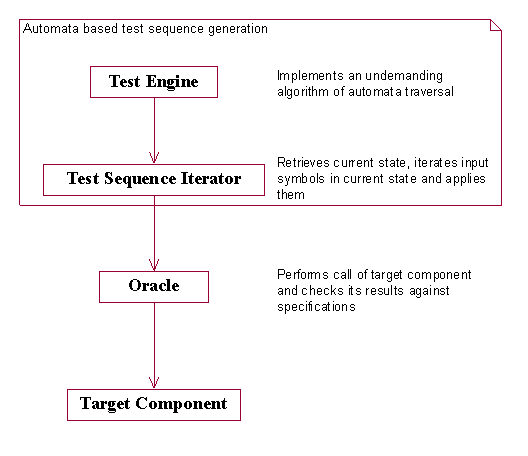
\includegraphics[width=\columnwidth]{basicarch.png}
\caption{Basic architecture of UniTesK test suite}
\label{fig:basicarch}
\end{center}
\end{figure}

So, the main idea of UniTesK testing technique is separation between test
sequence generation and behavior verification tasks. Test engine and
test sequence iterator are responsible for test sequence generation
and require only a part of description of an automaton under test --
the set of states and applicable input symbols for each state. Oracles
of target components are called during the work of test sequence
iterator's \texttt{call()} operation and, in turn, call the corresponding target
operations and perform the verification of the behavior of these operations
against their specifications. 

Figure~\ref{fig:basicarch} shows the basic architecture of UniTesK
test suite. We do not consider here auxiliary components responsible
for trace gathering and run-time test support, because they have no
any UniTesK specifics. 

The test engine component is a predefined part of a test suite. There
are several such components, but the test developer do not need to
write them manually; an existing
one shall be used. Oracles are supposed to be generated automatically from
specifications, which in turn are always developed by hand.

The test sequence iterator shall provide all possible input symbols for
each state of the automaton under traversal. Remember, that this
automaton is constructed from the behavior of the system under test
and some coverage criterion, or coverage of all possible test
situations. Input symbol of the automaton under traversal corresponds
to some class of possible inputs for the system under test. 

\subsection{Test Coverage Criteria}

An arbitrary coverage criteria can be described by a number of predicates
depending on the target operation identifier and a list of its input
parameters. Each of these predicates determines one element of the
coverage. The set of predicates, describing the coverage based on the
structure of implementation or specification could be extracted from
them, but it is not easy task in the common case. To facilitate this work
the UniTesK technology requires the specification designer to emphasize
the basic partition of the specified operation domain by means of
special constructs, branch function. The elements of this basic
partition correspond to subdomains where the specified operation has
substantially different functionality. 

But how can the predicates describing coverage be used? In most simple
cases the corresponding boolean predicates can be solved to
produce automatically the set of test cases that ensures the test
coverage needed. Unfortunately, it is impossible in general -- because the
predicates obtained can be unsolvable by any algorithm, or, if we
remember that all the data in real computers are from some finite
sets, they are practically unsolvable due to enormous amount of time
needed for that. 

Thus, the general case solution should allow the test designer to
facilitate test case generation with some handmade components of test
system, which are called iterators in UniTesK. However the predicates
defined above do remain useful. They can be used to filter the test
cases provided by iterators, and, so, iterators need not to be very
precise -- it is enough, if an iterator used for some component under
test provides a wide range of possible inputs, including at least one
representative of each coverage class. In UniTesK test development
technology the predicates describing the target coverage, for example,
the coverage extracted form the structure of specifications, are used
to generate a special kind of test system components called coverage
trackers. 

Such a coverage tracker is used as a part of test sequence iterator
component. It determines the element of the target coverage
corresponding to a call of the target operation generated by iterator
and checks whether this element has been covered before during the
test. If not, this call is considered as the next unapplied input
symbol, and the tracker marks the corresponding coverage element as
covered (because the test engine actually performs this call later),
otherwise the coverage tracker calls the iterator for the next call. When
all the elements of the coverage are covered, the coverage tracker
reports that there are no unapplied input symbols and the test can be
completed. 

\subsection{The Test Sequence Iterator}

Other functionality of test system iterator is represented by operations
\texttt{getState()} and \texttt{call()}. When we consider the coverage
criteria based only on coverages of component's operations domains,
the latter operation can be generated in general case. For most testing
tasks it is enough, but sometimes, when we need to cover some specific
sequences of calls of target operations, we should write part of the
second operation by hands, and for this reason this possibility exists
in UniTesK technology.

\begin{figure}[tbh]
\begin{center}
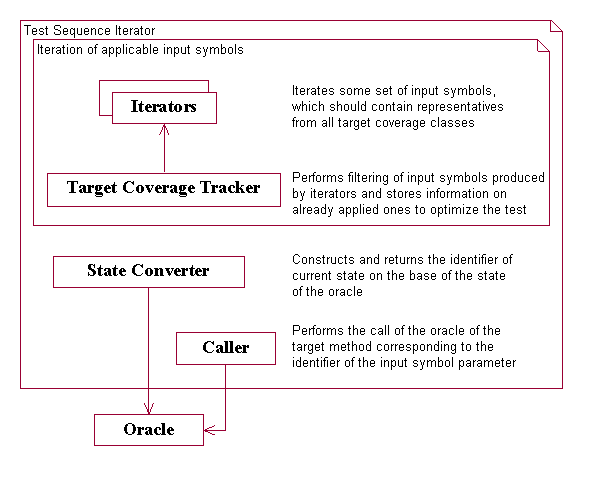
\includegraphics[width=\columnwidth]{testseqiter.png}
\caption{Typical structure of test sequence iterator component}
\label{fig:testseqiter}
\end{center}
\end{figure}

Figure~\ref{fig:testseqiter} shows the structure of mechanism
iterating applicable input symbols used in UniTesK. 

As illustrated above, test sequence iterators have a complex
structure. The bulk of which is usually generated automatically --
target coverage trackers and caller implementing \texttt{call()}
operation. Sometimes callers need a bit of manual code and sometimes
the state converter component and iterators can also be generated. To
provide a coherent description of all the parts of test sequence
iterator UniTesK operation proposes a form of test scenario, which
partially generated and partially written by hand. Test scenario
serves as a source for test sequence iterator generation. For more
detailed description of the structure of test scenarios see below. Our
experience shows that the ratio of generated code size to manual code
size in test sequence iterator component is usually more than 4:1.

\subsection{Use of Design Patterns}

One more important point of UniTesK test suite architecture is the use
of adapter pattern to bind
specification and implementation of the target component. For
historical reasons we call adapters, which have specification
interface and implement it on the base of the implementation under
test, mediators. 
 
To be able to produce reusable and repeatable tests is crucial for
industrial test development technology. UniTesK supports reusability
of tests and specifications by using more abstract specifications,
which can be applicable to several versions of the target
component. To perform a test in such a situation we should have
something to bind the immutable specification with a changing
implementation. One of the simplest and at the same time most flexible
solutions is to use a mediator component having the interface of
specification and implementing it with the help of
implementation. Such an approach allows us to change the level of
abstraction of specifications and tests developed with the help of
UniTesK technology in almost arbitrary way. 

Along with implementation of the specification interface, a mediator is
responsible for synchronization of its state as it is defined in
specifications with the state of the implementation, which can have
an entirely different form. This is important to support open state
testing, which assumes that on every step (between two calls of target
operations) we can determine exactly what the current state of the
component is. 

\begin{figure}[tbh]
\begin{center}
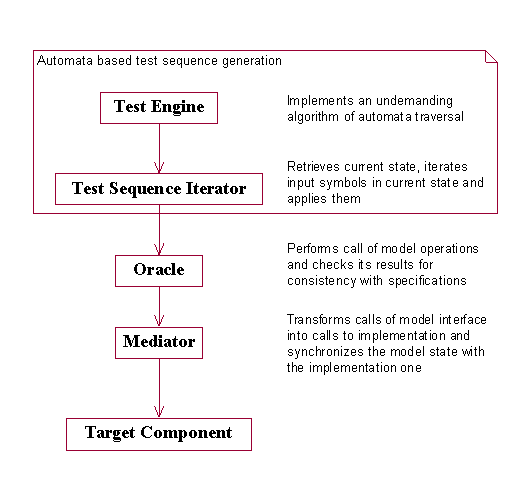
\includegraphics[width=\columnwidth]{uniteskarch.png}
\caption{Complete architecture of UniTesK test suite}
\label{fig:uniteskarch}
\end{center}
\end{figure}

Figure~\ref{fig:testseqiter} demonstrates the complete set of the main
components of UniTesK test suite architecture. However auxiliary
components of test suite responsible for tracing and run-time test
support have been left out.

Mediator components are usually written by hand. This fact increases
the total size of manual work, but in return we have the possibility
to develop really reusable specifications and tests, sometimes
comprising the complete and ready-to-use suite for regression
testing. 

\section{VDM++TesK Test Suite Architecture}

\subsection{Relating UniTesK to VDM++TesK}

This section will demonstrate how the VDM++TesK test suite
architecture corresponds to that of UniTesK described above. 

The VDM++TesK test suite architecture is implemented as a collection of
classes with well-defined functionality. Each
component of the UniTesK test suite presented on
Figure~\ref{fig:basicarch} and Figure~\ref{fig:testseqiter}
corresponds to a class or a group of classes (or even to parts of
classes). Each class of the VDM++TesK test suite belongs to one of
three kinds depending on its origin. Such kinds are: 

\begin{itemize}
\item hand-made; 
\item pre-built; and 
\item generated. 
\end{itemize}

Abstracting from a few details, a class diagram of the VDM++TesK test
suite is as shown in Figure~\ref{fig:TSclassdia}.

\begin{figure}[tbh]
\begin{center}
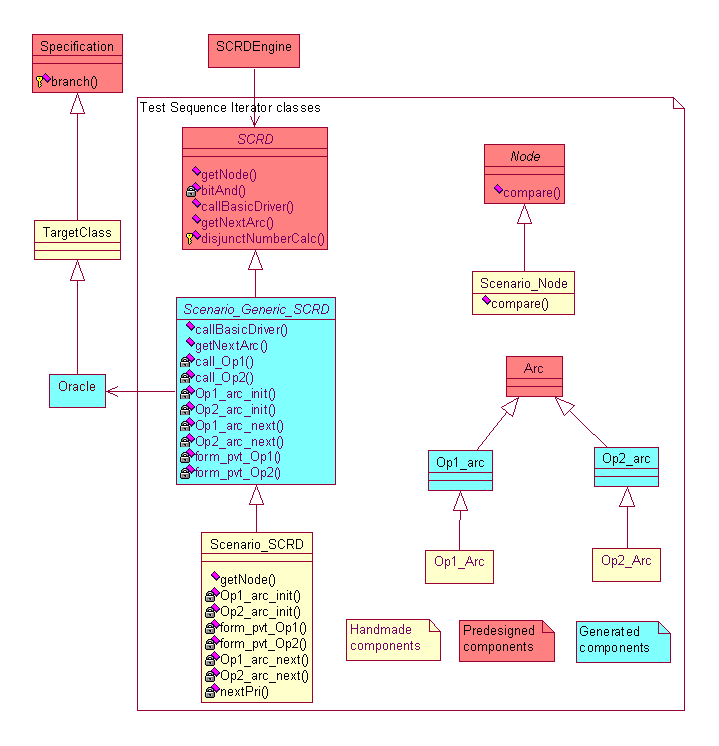
\includegraphics[width=\columnwidth]{TSclassdia.png}
\caption{VDM++TesK Test Suite Class Diagram}
\label{fig:TSclassdia}
\end{center}
\end{figure}

For each of the components in the UniTesK framework the classes in the
VDM++TesK solution will be explained below:

\begin{description}
\item[Target Component] in VDM++TesK is presented by one or more VDM++
classes, which functionality should be tested. On the class diagram it
is presented by the \textsf{Target Class}.

\item[Oracle component] corresponds to the class of the VDM++TesK test
  suite called \textsf{Oracle class}. It is aimed at checking
  conformance of behavior of the target operations (operations of the
  target class(es)) with their specifications. In the \textsf{Oracle
  class}, for each target operation, a operation with identical
  signature is defined (as it is seen on the class diagram, the
  \textsf{Oracle class} is inherited from the target class, so oracle
  operations override the target ones). In case of correct behavior of
  the corresponding target operation (i.e.\ if conformance is held),
  the result of the oracle operation (i.e.\ its return values and
  values of object instance variables) coincides with the target
  operation result. Otherwise, the oracle operation raises an
  exception depending on the kind of a discrepancy (e.g.\ if class
  invariant or pre- or postcondition is violated).

The \textsf{Oracle class} is automatically generated basing on the
target class formal specification written in VDM++.

\item[Test Engine component] is implemented by the \textsf{Test Engine class}
  of the VDM++TesK test suite. This class implements an algorithm of
  the FSM traversal. In VDM++TesK, such an algorithm is intended for
  deterministic mutual connected automata traversal. The \textsf{Test
  Engine class} is pre-built and uses the interface described above
  for automata traversal.

\item[Test Sequence Interator component] is implemented by several
  classes that are combined into a group called \textsf{Test Sequence
  Iterator} classes in Figure~\ref{fig:TSclassdia}. Below this
  component will be examined in more detail.
\end{description}

\begin{figure}[tbh]
\begin{center}
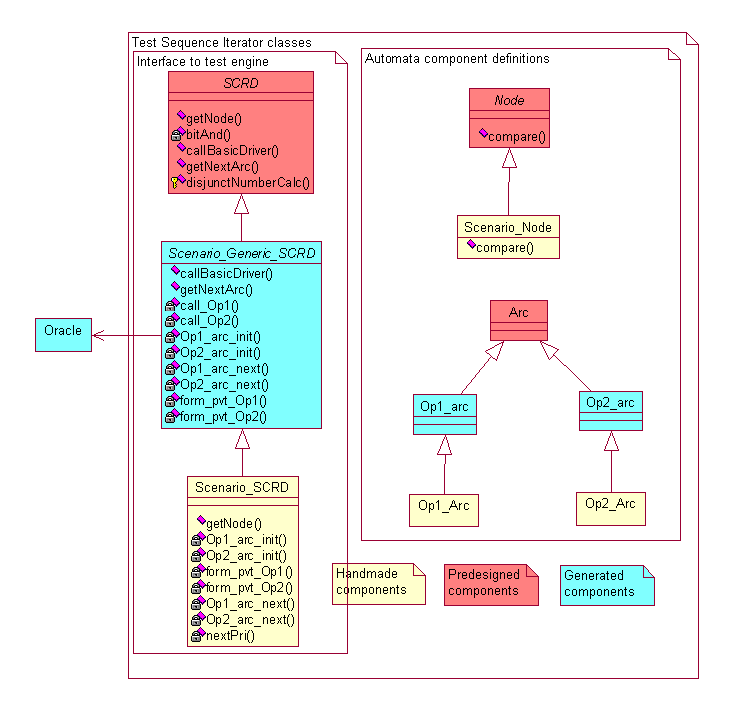
\includegraphics[width=\columnwidth]{TSIclassdia.png}
\caption{Test sequence iterator class diagram}
\label{fig:TSIclassdia}
\end{center}
\end{figure}

\subsection{Test Sequence Iterators}

The architecture of the test sequence iterators in UniTesK is presented in
Figure~\ref{fig:testseqiter}. The class diagram of the test sequence
iterators in VDMTesK is presented in
Figure~\ref{fig:TSIclassdia}.

The classes in the VDM++TesK solution are explained below:

\begin{description}
\item[\texttt{SCRD}:] Pre-built class that contains data and
operations for test sequence iteration that do not depend on a concrete
  collection of operations to be tested.
\item[\texttt{Scenario Generic SCRD}:] Class that is generated for concrete
  operations testing and aimed at test sequence iteration.  
\item[\texttt{Scenario SCRD}:] Hand-made class that contains data 
  and operations for test sequence iteration that cannot be
  generated automatically and must be written manually.
\item[\texttt{Node}:] Base class for FSM state identifier that is pre-built. 
\item[\texttt{Scenario Node}:] Handmade class for FSM state identifier
  for concrete test scenario. 
\item[\texttt{Arc}:] Base class for FSM input symbols that is pre-build.
\item[\texttt{op1\_arc, op2\_arc}:] FSM input symbols classes that are
  generated for each operation tested by this scenario.  
\item[\texttt{op1\_Arc, op2\_Arc}:] Hand-made FSM input symbols
  classes. Such class is defined only if the input symbol for the
  corresponding tested operation should contain additional information
  (see below).  
\end{description}

Classes of the Test Sequence Iterator can be grouped in the following manner:

\begin{itemize}
\item The \texttt{SCRD, Scenario Generic SCRD, Scenario SCRD} classes
  provide interface required for automata traversal by Test Engine
  that, in fact, performs testing.  
\item The \texttt{Node, Scenario Node, Arc, op1\_arc, op2\_arc, op1\_Arc,
  op2\_Arc} classes provide definitions of automata
  components (see above), namely nodes and arcs.  
\end{itemize}

\subsection{Test Iteration and Test Coverage}

The function of the Iteration of applicable input symbols group is to
deliver the next input symbol in the current state, which has not been
applied yet during this traversal. This task can be divided into two
parts: 

\begin{itemize}
\item iteration of input symbols (this task is solved by components
of Iterators group) and 
\item its filtration based on test coverage that is
already performed (Test Coverage Tracker component). 
\end{itemize}

The input symbols iteration is implemented by \texttt{<op
name>\_init()} and \texttt{<op name>\_next()} operations that are
defined in the hand-made class \texttt{Scenario SRCD} for each tested
operation.

Operations for the input symbols filtering are generated automatically
and defined in the generated class \texttt{Scenario Generic
  SCRD}. Moreover, these operations use information about test
coverage criteria that is automatically obtained from the
specification and is defined in the oracle class (see above). These
operations use a conversion of input symbols to input parameters of the
corresponding target operation. Operations for such conversions are
developed manually and defined in the \texttt{Scenario SRCD} class. 

When the \texttt{Test Engine} requests the next input symbol, it calls
\texttt{getNextArc()} operation of the \texttt{Scenario Generic SCRD}
class, and this operation, in turn, uses \texttt{<op name>\_init()}
and \texttt{<op name>\_next()} operations described above. 

The state converter component is implemented by the \texttt{getNode()}
operation defined in the hand-made class \texttt{Scenario SRCD}. Its
responsibility is to construct the FSM state identifier based on the
current state of the target system. This state can be obtained from an
object (or objects) of the oracle class (or classes).

The caller component is intended to impact the FSM under traversal with an
input symbol, what corresponds to the a call to the operation of the oracle
class with parameters defined by this input symbol. In the VDM++TesK
test suite, this component is presented with the
\texttt{callBasicDriver()} operation, which is generated automatically
and defined in the \texttt{Scenario Generic SCRD} class. This operation
uses operations named \texttt{call\_...()} that are generated for each
tested operation. These operations convert an input symbols to parameters of
the corresponding target operation and call that operation for the object of
oracle class. Operations for such conversion are manually defined in the
\texttt{Scenario SCRD} class and called the \texttt{form\_pvt\_...()} 
operation. In most cases, this collection of actions performed by
generated operations \texttt{call\_...()} is sufficient for testing,
however, test designer can redefine it if necessary.

Detailed description of test suite classes interfaces can be found in
Appendix~\ref{app:testclasses}. 

Notice that the mediator component shown on
Figure~\ref{fig:uniteskarch} is not implemented in the VDM++TesK test
suite. As it was mentioned above, mediators are used for binding
between the target system and its model. In VDM++TesK, it is assumed
that the target system structurally coincides with its model. In this
case, mediators are not needed. In case when it is necessary to
separate a system and a model, test designer can use
mediators. However, description of the mediators development is out of
scope in this document. 

In the part of the UniTesK technology description dedicated to the test
coverage, it was said that a designer can use nonstandard test coverage
criteria. However, this possibility is absent in
VDM++TesK. Moreover, the only coverage criterion supported is the
criterion based on postcondition branches coverage. 

\section{Test Development}

In this section a description of the test development process is
provided. A small example will be used to explain the steps of the
development, and a test suite for a class implementing a priority
queue will be used. The full list of the VDM++ files composing this
test suite can be found in Appendix~\ref{app:testclasses}.

The VDM++TesK test development process has the following steps:

\begin{enumerate}
\item constraints are developed for the target classes and operations,
  i.e.\ their formal specifications are written;  
\item groups of the operations are selected to be tested simultaneously,
  and for each such group a test scenario is developed.  
\end{enumerate}

\subsection{Specification Development}

Constraints of the target class are defined in the same class. A
specification class (i.e.\ target class with constraints defined in it)
should be a subclass of the pre-built class
called \texttt{Specification}, where function \texttt{branch} is
defined. 

In VDM++TesK, the following constraints are used:

\begin{enumerate}
\item Class invariants (constraints on the instance variables that are
  common for all operations of this class)  
\item Constraints for each operation
  \begin{enumerate}
  \item Instance variables access description 
  \item Operation preconditions 
  \item Operation postcondition 
  \end{enumerate}
\end{enumerate}

VDM++TesK does not support semantics of the specification classes
inheritance. The inheritance from a specification class implies only
explicit definitions inheritance (i.e.\ data and explicit operations
definitions). Base class constraints are ignored. 

See for example the \texttt{PriorityQueue} class on
page~\pageref{cla:prioque}. 

\subsection{Class invariants}

For the invariants definition, the standard VDM++ expressions
is used after instance variables. 

All expressions used in the invariant definition should be executable
by the VDM++ interpreter. 

\subsection{Constraints for each operation}

Operations for which postcondition is required should be defined using
the VDM++computable "extended explicit operation definition". This is
the only way to combine both its explicit implementation and access to
instance variables in the single operation declaration. 

\subsubsection{Instance variables access definition}

The instance variables access definition describes how the operation uses
the class's instance variables. 

For an access definition, the standard VDM++ construct "externals" is used.

See access definitions for operations \texttt{PriorityQueue`enqp}
(page~\pageref{op:enqp}), 
\texttt{PriorityQueue`enq} (page~\pageref{op:enq}), 
\texttt{PriorityQueue`deq} (page~\pageref{op:deq}),
\texttt{PriorityQueue`size} (page~\pageref{op:size})
and \texttt{PriorityQueue`isEmpty} (page~\pageref{op:isEmpty}).

\subsubsection{Operation preconditions}

A precondition describes the operation's condition of applicability
according to its input values and the object's state. 

A precondition is defined using a predicate after the VDM++ keyword ``pre".

An expression used as the precondition should be executable by the
VDM++ interpreter. 

See the precondition definition for the operation
\texttt{PriorityQueue`enqp} on page~\pageref{op:enqp}.

\subsubsection{Operation postcondition}

A postcondition defines a relation between the operation's input
parameters and the object's pre-state (the values of instance
variables before the operation invocation), and the operation's output
values and the object's post-state (the values of the instance
variables after the operation's completion). 

A postcondition is defined using a predicate after the VDM++ keyword ``post".

In VDM++TesK, the so-called branch coverage is used as a coverage
criterion. To enable VDM++TesK to elicit test coverage
criteria, so-called branches should be denoted in the
postcondition. Each branch describes one of the alternative behaviors
of the operation. 

To denote each branch, the postcondition must be defined using the VDM++
``if expression". Each branch must be marked with a name
that is unique for the given operation. 

\begin{lstlisting}
  if p1 then branch("branch #1") and post1
  elseif p2 then branch("branch #2") and post2
  ...
  elseif pn-1 then branch("branch #n-1") and postn-1
  else branch("branch #n") and postn
\end{lstlisting}

The predicates \texttt{p1 ... pn-1} determine the partitioning of the input
parameters space. In such predicates, only the pre-values should be
used -- the operation's input parameters and the object's instance
variables in the pre-state. The constraints \texttt{post1 ... postn} determine
the operation's behavior correctness in each of the alternatives.

If the postcondition can't be divided into more than one branch, it
should be written in the following manner: 

\begin{lstlisting}
  branch("single branch") and post
\end{lstlisting}

An expression used for the postcondition definition should be
executable by the VDM++ interpreter. 

See the postconditions for the operations \texttt{PriorityQueue`enqp}
(page~\pageref{op:enqp}), 
\texttt{PriorityQueue`enq} (page~\pageref{op:enq}), 
\texttt{PriorityQueue`deq} (page~\pageref{op:deq}),
\texttt{PriorityQueue`size} (page~\pageref{op:size}) and 
\texttt{PriorityQueue`isEmpty} (page~\pageref{op:isEmpty}).

\subsection{Test scenario development}

A test scenario development starts with the definition of a group of
operations which will be tested by it. In most cases, all operations of a
class naturally form such group. However, sometimes this approach of
grouping makes test execution time-consuming. In this case, operations
may be grouped according to such considerations as use cases. In any
approach, a group should be complete in the following sense. There
should not be "irreversible'' impacts to the tested system, i.e. the
system can be returned to its initial (the particular) state from any
state using only operations from this group. 

The operations group is described by the list of their qualified named
(\texttt{<class name>`<op name>}). Based on its description, the
VDM++TesK tools generate the classes required for test sequence
iteration (about these classes, see VDM++TesK test suite
architecture). Then test developer should write the following handmade
classes:

\begin{enumerate}
\item FSM state identifier; 
\item Classes that describe FSM input symbols; and 
\item Test sequence iterator class. 
\end{enumerate}

\subsubsection{FSM state identifier}

As mentioned above, a set of target system states can be divided
into equivalence classes. A state identifier determines the membership
of the corresponding system state in a particular equivalence class,
or, in terms of FSM, in its particular state. A FSM state
(and, hence, state identifier) may correspond to several target system
states. 

Class describing state identifier is derived from the pre-built class
called \texttt{Node}. In this class test developer should define data
that determines state of the tested FSM. For example, for the priority
queue, such state is described as a mapping from priorities existing
in the queue to the number of elements with such priority. 

Moreover, in this class, an operation compare should be defined as:

\begin{lstlisting}
  compare : Node ==> bool
\end{lstlisting}

\texttt{n1.compare(n2)} returns \texttt{true} if and only if
\texttt{n1} and \texttt{n2} are identifiers of the same automaton
state (i.e.\ they correspond to target system states belonging to the
same equivalence class). 

See class \texttt{PQueue\_Node} on page~\pageref{clapquenode}.

\subsubsection{Classes that describe FSM input symbols}

An impact on the FSM by an input symbol is a call to the corresponding
target operation. For each operation under test, an empty class (declaring
no data) is automatically generated. Such class corresponding to a
operation \texttt{<op name>} is called \texttt{<op
  name>\_arc}. During the test execution, the input symbol's
membership in one of such classes determines the operation to be called,
and parameters of this operation are determined using the corresponding
conversion operation (see below). Thus, in a class describing a FSM
input symbol, the test developer should declare data required for such
conversion. This data should be defined in class inherited from the
generated class. 

For example, consider the handmade input symbol class
corresponding to the \texttt{enqp} queue operation
(\texttt{PriorityQueue\_enqp\_Arc}). In this case, different input
symbols correspond to the enqueing items with different priorities. 

In case when it is not necessary to test with certain parameters of a
operation, the test developer does not need to define such
classes. Notice, that the \texttt{form\_pvt\_<op name>()} operations
still should be defined for such operations.

It should be noticed that in VDM++TesK FSM should be deterministic,
i.e.\ any input symbol applied in the particular state should lead the
FSM to the same state regardless of the previous transitions. 

\subsubsection{Test sequence iterator}

In this class, the following should be defined:

\begin{enumerate}
\item Oracle objects initialization; 
\item Acquisition of the FSM state identifier; 
\item Operations for the input symbols iteration (for each target operation); 
\item Operations for conversion of input symbol into operation's
parameters; and 
\item Operations for calling the oracle. 
\end{enumerate}

See \texttt{class SCRD\_PQueue} on page~\pageref{cl:SCRD_PQueue}.

\paragraph{Oracle objects initialization}\mbox{}\\

In the class-iterator, objects of tested classes oracles are
defined. If any initialization for oracles is needed, a operation for
such initialization should be defined in the class-iterator. 

This operation should be called \texttt{<scenario name>\_init} and can
have parameters required for the initialization. 

\paragraph{Acquisition of FSM state identifier}\mbox{}\\

The test developer should declare operation for state identifier
construction basing on the target system's current state. Values of
the tested class instance variables can be obtained from the
corresponding oracle object (references to such objects are stored in
the variables called \texttt{oracle\_of\_<class name>}). 

See operation \texttt{SCRD\_PQueue`getNode} on page~\pageref{op:getNode}.

\paragraph{Operations for the input symbols iteration}\mbox{}\\

For each tested operation, a pair of operations must be defined -- an
operation that constructs a first input symbol to be applied in the
current state and a operation that constructs a next input symbol based
on the previous one. 

\begin{description}
\item[\texttt{<class name>\_<op name>\_arc\_init}:] 
This operation yields a pair where the first component is the first
input symbol for the current state. A false value in the second
component means that the given target operation should not be
invoked in this state.
\item[\texttt{<class name>\_<op name>\_arc\_next}:] 
This operation computes the next input symbol according to the previous
one. A false value of the second return component means that the iteration
of operation's input symbols for the current state is completed.  
\end{description}

For operations with no input parameters, these operations shall not be defined.

See operations \texttt{PriorityQueue\_enq\_arc\_init}
(page~\pageref{op:PQenq_arc_init}), 
\texttt{PriorityQueue\_enqp\_arc\_init} (page~\pageref{op:PQenqp_arc_init}),
\texttt{PriorityQueue\_enq\_arc\_next}
(page~\pageref{op:PQenq_arc_next}) and
\texttt{PriorityQueue\_enqp\_arc\_next} (page~\pageref{op:PQenqp_arc_next}). 

\paragraph{Operations for conversion of input symbol into operation's
  parameters}\mbox{}\\ 
 
For each tested operation, an operation shall be defined that converts
an input symbol into this operation's input parameters. 

For each tested operation, a structure is defined that holds values of
this operation's input parameters, and an operation that converts the input
symbol into such a structure. 

Type of such structure is named \texttt{pvt\_<class name>\_<op
  name>}. Types and names of its fields and their order are equal to
types and names of the corresponding operation's formal parameters. 

See types \texttt{pvt\_PriorityQueue\_enq} and
\texttt{pvt\_PriorityQueue\_enqp} (page~\pageref{ty:pvt_PQ_enq}). 

The conversion operations has the following signature:

\begin{lstlisting}
form_pvt_<class name>_<op name>: 
     <class name>_<op name>_arc ==> 
     pvt_<class name>_<op name>
\end{lstlisting}

Notice, that these operations and types are not defined for tested
operations without input parameters. 

See \texttt{form\_pvt\_PriorityQueue\_enq} and
\texttt{form\_pvt\_PriorityQueue\_enqp} (page~\pageref{op:form_pvt_PQ_enq}).

\paragraph{Operations for oracle calling}\mbox{}\\

In the most cases, these operations can be generated
automatically. However, sometimes for parameter iteration, output of
target operations is required, or sequence of operations should be called as
a reaction on a single input symbol. In such cases, these operations shall
be defined manually. 

\begin{lstlisting}
call_<class name>_<op name>: 
     <class name>_<op name>_arc ==> bool
\end{lstlisting}

These operations return a boolean value that indicates successful oracle
invocation (i.e.\ that the oracle had found no errors).  

In the given example, these operations are generated automatically. See
\texttt{call\_PriorityQueue\_enqp}, \texttt{call\_PriorityQueue\_enq},
\texttt{call\_PriorityQueue\_deq}, \texttt{call\_PriorityQueue\_size}
and \texttt{call\_PriorityQueue\_isEmpty} (page~\pageref{op:call_PQ_ops}). 


\section{Test execution and analysis}

Now, when the test suite is developed, the test suite can be executed.

\subsection{Test execution}

To run the test, the FSM traversal algorithm should be executed with
the FSM described by the test scenario. 

An object of the \texttt{SCRDEngine} class shall be created and
initialized with test sequence iterator class using its constructor,
and subsequently its main operation shall be invoked.

The following will run the test developed for the priority queue example.

\begin{lstlisting}
  new SCRDEngine(new SCRD_PQueue()).main()}
\end{lstlisting}

\subsection{Test trace and its analysis}

During an oracle execution, it traces information about the test
coverage. After the test is executed, this information serves as a
base for determining the test results -- what test coverage has been
performed and whether there were any errors. In addition the test
trace can be used for exploring errors.

For the present time, test trace analysis must be done manually.

See example of test trace in Appendix~\ref{sec:trace}.

\appendix

\newpage
\bibliographystyle{newalpha}

\bibliography{dan}

\newpage
\section{Setting up VDMTesK}

\subsection{Software requirements}
\begin{itemize}
\item vdmtesk package
\item \href{http://java.sun.com}{j2sdk1.4.2\_16}
\item \href{http://www.eclipse.org/downloads/}{Eclipse Classic}
\item \href{http://fmvdm.org/}{The VDM++ or VICE
version of VDMTools}
\item \href{http://ant.apache.org/bindownload.cgi}{Ant}
\item VDMTesK source files
\end{itemize}

\subsection{Installation}

\subsubsection{Installing J2SDK}
The j2sdk package is an executable file. Double click on the installation file, and follow the instructions.


\subsubsection{Installing Eclipse}
After download the eclipse classic version, unpack it to a folder (e.g. eclipse).

\subsubsection{Installing VDMTools}
The VDM version needed is the VDM++ toolbox. After download it, double click on the executable and follow the instructions.

\subsubsection{Installing Ant}
After doing the download and unpack it, follow these steps:
\begin{enumerate}
\item Click \textbf{Start}. Click with the right bottom of the mouse in \textbf{My Computer}.
\item Click Properties $\rightarrow$ Advanced $\rightarrow$ \textbf{Environment variables}.
\item The user should have the following environmental variables:
\begin{verbatim}
Variable: ANT_HOME
Value: the path to the directory ant

Variable: ANT_OPTS
Value: -Dhttp.proxyHost=<proxy_settings> -Dhttp.proxyPort=<port>

Variable: JAVA_HOME
Value: the path to jdk1.5.0_13
\end{verbatim}
The system variable (Path) should have the following paths:
\begin{verbatim}
Path to \ant\bin
Path to jdk1.5.0_13\bin
\end{verbatim}
\end{enumerate}
If any problem appear, please see the installation notes in the ant
\texttt{INSTALL} file. 
\subsubsection{Installing VDMTesK}
\begin{enumerate}
\item Unzip the \texttt{vdmtesk.zip} file. In this tutorial, it is assumed that the folder will be called \texttt{vdmtesk}.
\item Install all the software refered above.
\item Run '\texttt{ant setup}' (from \texttt{vdmtesk} directory) to download \texttt{javacc}, using the Windows command prompt.
\item Run '\texttt{ant distr.jar}' (from \texttt{vdmtesk} directory) using the Windows command prompt to generate Java code for javacc parsers (\texttt{*.jj}),
 AST abstract syntax tree (\texttt{*.ast}), compile Java and pack classes to jar.\\
If you need to perform individual steps, run the following commands sequentially:
\begin{itemize}
\item \texttt{ant AST.jj}
\item \texttt{ant VDM.jj}
\item \texttt{ant compile.ast.java}
\item \texttt{ant VDM.ast}
\item \texttt{ant compile.java}
\end{itemize}
If any command fails, besides the last one, they were not installed
properly or it is being used another Operating System besides Windows.
If that is the case, note that the operating system can be case
sensitive; maybe it is necessary to run these commands without capital
letters.  If the last one fails, it means that the Java code has
errors: probably there are some dependencies missing (e.g.\ \texttt{JMK} or
\texttt{ToolBoxAPI}) which will be solved in the next steps.
\item Open the file \texttt{.tesktool} and change the variables
\texttt{toolbox.path} and \texttt{user.dir}.  
The \texttt{toolbox.path} must have the path to the VDM++ gde executable and
the \texttt{user.dir} must have the path to the vdmtesk home directory. Here it
is an example:
\begin{verbatim}
toolbox.path C:\\The VDM++ Toolbox v8.2b\\bin\\vppgde.EXE
user.dir C:\\vdmtesk
\end{verbatim}
\item Open Eclipse and create a new java project. Note that the workspace must have a different path from where is the vdmtesk.
Give a name to the project and choose "\texttt{Create project from existing source}". Browse the directory \texttt{vdmtesk}.
Click Next.
Click in the check box to "\texttt{Allow output folders for source folders}". Click Finish.\\
\item It is necessary to insert 2 new libraries:
\begin{enumerate}
\item Inserting the library JMK\\
Click Build path $\rightarrow$ Add libraries $\rightarrow$ User Library $\rightarrow$ Next $\rightarrow$ User libraries $\rightarrow$ New\\
Give the name JMK\\
Click Add JARs and browse vdmtesk/jar/jmk.jar
\item Inserting the library ToolBoxAPI\\
Similar process:\\
Click New\\
Give the name ToolBoxAPI\\
Click Add JARs and browse vdmtesk/jar/ToolBoxAPI.jar\\
\end{enumerate}
If the standard library is different from the j2sdk mentioned in the Installation section, it must be changed.
To do that, follow the following steps:
\begin{itemize}
\item Click with the right bottom of the mouse over the name of the project and click Build Path $\rightarrow$ Configure Build Path\\
\item Select the System Library and click Edit. Then, click \textbf{alternate jre} and choose the right jre system library. At the
end click Finish $\rightarrow$ Ok.
\end{itemize}
\item There should be no errors in the project, now. Assuming that, click with the right bottom of the mouse
over vdmtesk (or the name of the project) and click Source $\rightarrow$ Clean up $\rightarrow$ Next $\rightarrow$ Finish
\item Click Run $\rightarrow$ Open Run Dialog $\rightarrow$ Java Application. Complete the form like this:
\begin{verbatim}
Project: The name given to the project
Main class: ru.ispras.redverst.vdmtesk.Main
\end{verbatim}
\item Click run
\end{enumerate}

\newpage
\section{VDM++TesK test suite classes}

\subsection{Target class}

The target class is the VDM++ class which functionality that shall be tested.

\subsection{Oracle}

Based on a formal specification an \texttt{Oracle} class is generated.

The \texttt{Oracle} class is inherited from the \texttt{Specification} class.

In an oracle, the following members are defined:

\begin{itemize}
\item Operations for checking of specification and implementation conformance 
\begin{itemize}
\item Operation for invariants checking ;
\item Operations for precondition checking; 
\item Operation-oracles that check postcondition; and 
\item Flags that determine whether to call oracle operation or not. 
\end{itemize}
\item Test coverage support 
\begin{itemize}
\item Filter operations; and 
\item Values that hold the number of branches in postconditions. 
\end{itemize}
\end{itemize}

Functionality of these components is described further below.

An \texttt{Oracle} class has the same interface as the corresponding class
under test.

\subsubsection{Operations for checking of invariants (\texttt{checkInv\_<class name>})} 

The operation for invariants checking (\texttt{checkInv\_<class name>})
This operation checks invariants of the class under test. It evaluates all expressions marked as class invariants, and throws an exception if one of them evaluates to false.

See \texttt{checkInv\_PriorityQueue} on page~\pageref{op:checkInv_PQ}.

\subsubsection{Operations for precondition checking (\texttt{<op name>\_pre})}

For each the target operation, the oracle class declares operation that
checks this operation's precondition.

See \texttt{enqp\_pre} (page~\pageref{op:OraclePQenqp}), 
\texttt{enq\_pre} (page~\pageref{op:OraclePQenq}), 
\texttt{deq\_pre} (page~\pageref{op:OraclePQdeq}),
\texttt{isEmpty\_pre} (page~\pageref{op:OraclePQisEmpty}) and 
\texttt{size\_pre} (page~\pageref{op:OraclePQsize}). 

\subsubsection{Operation-oracles that check postconditions (\texttt{<op
name>\_post})}

For each target operation, the oracle class declares an
operation-oracle. This operation is aimed at checking of a postcondition of
the corresponding target operation. The signature of such operation is
equivalent to the target operation signature. If the postcondition is
false, this operation throws an exception. 

In order to check a postcondition, an oracle saves values of instance
variables that marked in signature as ``written'' by the target
operation, before the target operation execution.

See \texttt{enqp\_post} (page~\pageref{op:OraclePQenqp}),
\texttt{enq\_post} (page~\pageref{op:OraclePQenq}), 
\texttt{deq\_post} (page~\pageref{op:OraclePQdeq}),
\texttt{isEmpty\_post} (page~\pageref{op:OraclePQisEmpty}) and 
\texttt{size\_post} (page~\pageref{op:OraclePQsize}). 

Flags that determine whether to call oracle operation or not can be
defined. 
For each target operation, oracle class declares a flag -- a boolean
variable that determines whether to call the oracle operation (to check
postcondition) or not. 

See \texttt{test\_conf\_var} (page~\pageref{inst:test_conf_var}) and 
\texttt{test\_conf\_all} (page~\pageref{inst:test_conf_all}).

\subsubsection{Filter operations (\texttt{<op name>\_bnc})}

On basis of the coverage criteria information taken from the
specification, operations and data are defined in the oracle. 

For each target operation, the \texttt{Oracle} class declares a
filtering operation. Its input parameters are identical to the
parameters of the target operation. As a result, this operation
returns information about the test coverage equivalence class that
the current object state and input parameters corresponds to. In
particular, this operation returns an ordinary number of a
postcondition branch which will be covered.

See \texttt{enqp\_bnc} (page~\pageref{op:OraclePQenqp}), 
\texttt{enq\_bnc} (page~\pageref{op:OraclePQenq}), 
\texttt{deq\_bnc} (page~\pageref{op:OraclePQdeq}),
\texttt{isEmpty\_bnc} (page~\pageref{op:OraclePQisEmpty}) and 
\texttt{size\_bnc} (page~\pageref{op:OraclePQsize}). 

The \texttt{max\_bn\_<op name>} instance variable holds the number of
branches in postconditions. To measure test coverage performed based
on postcondition branches, the information about number of such
branches is required. In an oracle, values that holds a branch number
of corresponded operation are declared.

See \texttt{max\_bn\_enqp}, \texttt{max\_bn\_enq},
\texttt{max\_bn\_deq}, \texttt{max\_bn\_isEmpty} and
\texttt{max\_bn\_size} (page~\pageref{inst:test_conf_all}). 

\subsubsection{Execution of oracle interface operations}

As a result of an oracle interface operation call, the following actions
are performed. 

\begin{enumerate}
\item target operation precondition is checked; 
\item if the flag of oracle invocation for corresponded operation is turned
on, then the oracle operation is called. Otherwise, the parent
operation is called (i.e.\ operation's implementation); and
\item invariant checking is performed.
\end{enumerate}
 
The work of the oracle operation consists of the following actions:

\begin{enumerate}
\item values of instance variables marked as ``written" by operation are
saved in local variables;  
\item the operation under test is called; 
\item postcondition checking is performed (in postcondition, instance
variables in pre-state replaced with its saved values).  
\end{enumerate}

See \texttt{enqp} (page~\pageref{op:OraclePQenqp}), 
\texttt{enq} (page~\pageref{op:OraclePQenq}), 
\texttt{deq} (page~\pageref{op:OraclePQdeq}), 
\texttt{isEmpty} (page~\pageref{op:OraclePQisEmpty}) and
\texttt{size} (page~\pageref{op:OraclePQsize}). 

\subsection{Test sequence iterator}

The VDM++TesK test suite describes an FSM that tests operations of the
target classes. 

The following components are parts of the test sequence iterator:

\begin{enumerate}
\item The class that describes automaton state identifier; 
\item The classes that describe input symbols of FSM; and
\item The class-iterator of test sequence. 
\end{enumerate}

This components are partially generated and partially developed manually.

\subsubsection{Automaton state identifier}

The class that describes automaton state identifier defines the single
operation -- the \texttt{compare} operation.

This class is derived from the pre-build abstract class called
\texttt{Node} on page~\pageref{cla:node}. 

\subsubsection{FSM input symbols}

For each tested operation included in a test scenario, a class that
describes the FSM input symbols must be defined. 

Each such class is derived from the pre-build class named \texttt{Arc}.

\subsection{Test sequence iterator}

This class represents, in fact, a description of the FSM.

Its interface is described by the abstract class \texttt{SCRD}. It
defines the following operations: 

\begin{enumerate}
\item Acquisition of current FSM state identifier (\texttt{getNode}); 
\item Acquisition of next FSM input symbol (\texttt{getNextArc}); and 
\item Applying input symbol to FSM in its current state
(\texttt{callBasicDriver}).
\end{enumerate}
 
\paragraph{Acquisition of current FSM state identifier}\mbox{}\\

This operation constructs an FSM state identifier corresponding to the
target system's current state. It returns an object of the class
inherited from the class named \texttt{Node}. 

\paragraph{Acquisition of next FSM input symbol}\mbox{}\\

A test sequence iterator shall produce a next FSM input symbol based
on previous one that was applied to a FSM in the current state. 

As an input parameter, this operation gets an object of a class
inherited from the class \texttt{Arc}. This operation returns an
object of class inherited from class \texttt{Arc}.

\paragraph{Applying input symbol to FSM in its current state}\mbox{}\\

This operation takes a parameter that is a subclass of the
\texttt{Arc} class. Applying the input symbol to FSM is just invocation 
of the operation corresponded to this symbol with parameters determined by
it.

\subsection{Test engine}

In VDM++TesK, the algorithm of a FSM states traversal is implemented
by the pre-build class called \texttt{SCRDEngine}. 

The given algorithm intended only for determined FSM's traversal.

An object of the \texttt{SCRDEngine} class should be initialized by an
object of a \texttt{SCRD} class inheritor -- an object that represents
a test scenario. Such initialization is performed using the
\texttt{SCRDEngine} constructor.

\begin{lstlisting}
  SCRDEngine: SCRD ==> SCRDEngine
\end{lstlisting}

The traversal algorithm is launched using the \texttt{main} operation. 

\begin{lstlisting}
  main: () ==> ()
\end{lstlisting}

The 
launch of an entire test scenario can be combined in a single expression: 

\begin{lstlisting}
  new SCRDEngine(scrd).Main()
\end{lstlisting}

\subsection{Test trace support}

A test execution trace is supported by the class \texttt{Tracer}. This
class allows to put a trace both into a file and to the VDMTools console. 

Besides the standard trace support operations used by generated test
suite components, this class declares the \texttt{putTraceMessage} operation that
can be used for test scenario debugging. 

\begin{lstlisting}
  putTraceMessage : seq1 of char ==> ()
\end{lstlisting}

To make a test trace to be put into a certain file, the operation
\texttt{setOutFile} can be used: 

\begin{lstlisting}
  setOutFile : seq of char ==> ()
\end{lstlisting}

If this operation is called with empty string as a parameter, a test
trace will be put to the VDMTools console. 

\newpage
\section{Example of VDM++TesK technology application}\label{app:testclasses}

Class implemented priority queue has been chosen as example of
VDM++TesK application. 

\begin{description}
\item[\texttt{priority\_queue.vpp}:] 
Manually developed. Implementation and specification of target class 
\item[\texttt{queue\_item.vpp}:] 
Manualkly develoiped. Base class for queue items 
\item[\texttt{priority\_queue\_oracle.vpp}:] 
Generated file. Oracle class 
\item[\texttt{pqueue\_scrd\_gen.vpp}:] 
Generated file. Generated parts of test scenario 
\item[\texttt{pqueue\_scrd.vpp}:] 
Hand-made parts of test scenario 
\item[\texttt{scrd\_engine.vpp}:] 
 Test engine 
\item[\texttt{scrd.vpp}:] 
Pre-build (system) file. Base and auxiliary classes for test scenarios 
\item[\texttt{specification.vpp}:] 
Pre-build (system) file. Specification base class 
\item[\texttt{io.vpp}:] 
VDM++ library for I/O 
\item[\texttt{tracer.vpp}:] 
Pre-build (system) file. Class that provide support for test execution tracing 
\item[\texttt{testgens.vpp}:] 
Pre-build (system) file. Definitions for test coverage support 
%\item[\texttt{test\_trace}:] 
%Pre-build (system) file. Test trace 
\end{description}
 
Each of these classes are presented in the subsections below divided
into the categories:

\begin{enumerate}
\item Predesigned components;
\item Generated components; and
\item Handmade components.
\end{enumerate}

\subsection{Predesigned Components}

\subsubsection{The \texttt{Arc} and \texttt{EmptyArc} Classes}

\begin{lstlisting}
-- Abstract class for script driver arc of graph
class Arc
end Arc

-- Class for presentation of empty arc
class EmptyArc is subclass of Arc
end EmptyArc
\end{lstlisting}

\subsubsection{The \texttt{Node} Class}

\label{cla:node}
\begin{lstlisting}
-- Abstract class for script driver node presentation
class Node
    
operations

public compare: Node ==> bool
compare(node) == is subclass responsibility;

end Node
\end{lstlisting}

\subsubsection{The \texttt{Specification} Class}

\begin{lstlisting}
class Specification

functions

protected branch : seq1 of char +> bool
branch(-) == true;
        
end Specification
\end{lstlisting}

\subsubsection{The \texttt{SCRD} Class}

\begin{lstlisting}
-- Abstract class for script driver
class SCRD

types

-- Script driver option types
public finish_mode = <until_error> | <until_end>;

public tcp_test_mode = <for_each_prt> | <for_each_ec>;

public 
pvt_test_mode =   <for_each_pvt>
                | <for_each_branch>
                | <for_each_disjunct>
                | <for_each_disjunct_with_conc_if_opti>;

public pvt_estimation =   <pre_condition_is_false>
                        | <do_not_test>
                        | <imperatively_test>
                        | <see_ECI>;

/*                                                     */
/*  Possible returned pvt_estimation depended          */
/*  on pvt_test_mode                                   */
/*  -------------------------------------------        */
/*                                                     */
/*     pvt_test_mode = for_each_pvt                    */
/*  =>                                                 */
/*        pvt_estimation = pre_condition_is_false      */
/*     \/ pvt_estimation = imperatively_test           */
/*                                                     */
/*     pvt_test_mode = for_each_branch                 */
/*  =>                                                 */
/*        pvt_estimation = pre_condition_is_false      */
/*     \/ pvt_estimation = imperatively_test           */
/*     \/ pvt_estimation = see_ECI                     */
/*                                                     */
/*     pvt_test_mode = for_each_disjunct               */
/*  =>                                                 */
/*        pvt_estimation = pre_condition_is_false      */
/*     \/ pvt_estimation = imperatively_test           */
/*     \/ pvt_estimation = see_ECI                     */
/*                                                     */
/*     pvt_test_mode =                                 */
/*     for_each_disjunct_with_con_if_opti              */
/*  =>                                                 */
/*        pvt_estimation = pre_condition_is_false      */
/*     \/ pvt_estimation = do_not_test                 */
/*     \/ pvt_estimation = imperatively_test           */
/*     \/ pvt_estimation = see_ECI                     */
/*                                                     */
\end{lstlisting}

\begin{lstlisting}
-- TYPE FOR BC_PROC
public disTableType = map nat to nat;

instance variables
-- Test mode
public testMode: pvt_test_mode := <for_each_branch>;

-- Initialize tracer
public tracer: Tracer := Tracer`tracer;

operations

-- Evaluate node
public getNode: () ==> Node
getNode() == is subclass responsibility;

-- Get next arc
public getNextArc: ArcPrt*pvt_test_mode ==> ArcPrt * bool
getNextArc(in_arcprt, tm) == is subclass responsibility;

-- For given basic arc call basic driver
-- and returns next node, back-operation and verdict
public callBasicDriver: Arc ==> Node * Arc * bool
callBasicDriver(arc) == is subclass responsibility;

-- OPERATIONS FOR BC_PROC
bitAnd: nat*nat ==> nat
bitAnd(a, b) ==
  if (a <> 0) and (b <> 0) 
  then return (a mod 2) * (b mod 2) + 
              bitAnd(a mod 2, b mod 2) * 2
  else return 0;

protected disjunctNumberCalc:
   disTableType * seq of TESTGENS`KnownTermValue ==>
   disTableType * pvt_estimation * nat
disjunctNumberCalc(dis_table,termlist) == 
 (dcl cur_disjunct: nat := 0;
  dcl cur_disjnum : nat;
  dcl dis_tbl     : disTableType := dis_table;

  for i = 1 to len termlist by +1 do (
    cur_disjnum := if termlist(i).termValue 
                   then 2 
                   else 1;
    cur_disjnum := cur_disjnum * (2 ** (2 * 
                   termlist(i).termNumber));
    if bitAnd(cur_disjunct,cur_disjnum) = 0 
    then cur_disjunct := cur_disjunct + cur_disjnum
   );
  if cur_disjunct not in set dom dis_tbl 
  then dis_tbl := dis_table ++ 
        {cur_disjunct |-> card dom dis_tbl + 1};
  return  mk_(dis_tbl, <see_ECI>, dis_tbl(cur_disjunct))
 )
        
end SCRD
\end{lstlisting}
\subsubsection{The \texttt{SCRDEngine} Class}

\begin{lstlisting}
-- Basic engine of script drivers
class SCRDEngine

instance variables

-- Script driver
public scrd : SCRD;

-- List of tested states of object
public testedNodes : seq of TestedNode;
    
-- Path in graph - list of states of object under testing
public path : seq of PathNode;


operations

public SCRDEngine: SCRD ==> SCRDEngine
SCRDEngine(s) == 
 (scrd := s;

  testedNodes :=
    [new TestedNode().mkTestedNode(scrd.getNode(),
                                   new EmptyArc(),0,1)];

  path := [new PathNode().mkPathNode(1,new ArcPrt(),1)];
 );


-- Delete last node from path
delLastPathNode: () ==> ()
delLastPathNode () ==
  path := [path(i) | i in set{1,...,len path - 1}];

-- Make call basic driver
orientedCall: Arc ==> Node*Arc
orientedCall(cur_arc) ==
  let mk_(new_node,back_arc,verdict) =
      scrd.callBasicDriver(cur_arc)
  in (if not verdict then
         scrd.tracer.scriptTracerSuicide(
            "Oriented_call_:call_ returns bad verdict");
       return mk_(new_node,back_arc)
     );

-- Is the arrived node new?
isItNewNode: Node ==> nat
isItNewNode (n_node) == 
 (dcl tn_id: nat := 1;
  while (tn_id <= len testedNodes and
         not n_node.compare(testedNodes(tn_id).node))
  do tn_id := tn_id + 1;
    return tn_id
 );
\end{lstlisting}

\begin{lstlisting}
-- Update lists (testedNodes AND path):
-- add new node to path and tested list
updateLists: Node * Arc ==> ()
updateLists (new_node, back_arc) == 
 (dcl lastPathNode:   PathNode := path(len path);
  dcl backArcNum:     nat;
  dcl backNodeNum:    nat;

  backArcNum := if not isofclass(EmptyArc,back_arc)
                then lastPathNode.testedNodeId
                else 0;
  testedNodes := testedNodes ^
                 [new TestedNode().mkTestedNode
                         (new_node, back_arc,
                          backArcNum, len path + 1
                         )
                 ];
  backNodeNum := if not isofclass(EmptyArc,back_arc)
                 then len path
                 else len path + 1;
  path := path ^
          [new PathNode().mkPathNode
                              (len testedNodes,
                               new ArcPrt(),
                               backNodeNum
                              )
          ]
 );
\end{lstlisting}

\begin{lstlisting}
-- Go along back-arcs to path
goBackToPath: nat ==> nat
goBackToPath (tn_id) == 
 (dcl tested_node: TestedNode := testedNodes(tn_id);

   while  -- go along back-arcs to path
         tested_node.pathNodeId = 0
   do
     if  -- does back-arc exist?
         tested_node.backArcEndId = 0
     then (-- back-arc does not exist
           scrd.tracer.scriptTracerSuicide(
                 "MAIN_oriented_with_abstract_state_:" ^
                 "no back-arc in tested node");
           return tn_id
          )
     else  -- back-arc exists
          let -- movement along back-arc
              newTestedNodeId = tested_node.backArcEndId,
              mk_(newNode, -) = orientedCall
                                (tested_node.backArc)
          in (if -- is the result of movement
                 -- along back-arc right
                 not newNode.compare(testedNodes(
                             newTestedNodeId).node)
              then (-- the result of movement 
                    -- along back-arc is wrong
                    scrd.tracer.scriptTracerSuicide(
                     "MAIN_oriented_with_abstract_" ^
                     "state_:back-operation faults");
                    return tn_id
                   );
              tested_node := testedNodes(newTestedNodeId);
             );  -- End let - movement along back-arc
    -- End if - does back-arc exist
  -- End while - go along back-arcs to path

  -- Return index in path node list of first node
  -- along back-arcs which in path node list
  return tested_node.pathNodeId
 );
\end{lstlisting}

\begin{lstlisting}
-- Some node at path arrived this node index in path-list 
-- is newPathNodeId. newBackNodeId is index of back-node
-- of newPathNodeId node in path list.
-- if newBackNodeId is smaller than index of back-node of
-- last node of path then correct back-arcs and back-node
-- indexes of each node at path-list where point of 
-- returning to path is greater then newBackNodeId from 
-- end of path to newPathNodeId + 1
correctBackArcs: nat * nat ==> ()
correctBackArcs(newPathNodeId, testedLastArcEndId) == (
 (dcl newBackNodeId: nat := 
      path(newPathNodeId).backNodeId;

  if  -- is newBackNodeId smaller than index of back-node 
      -- of last node of path
      newBackNodeId < path(len path).backNodeId
  then (dcl pn:    PathNode;
        dcl tn:    TestedNode;
        dcl tn_id: nat;
        dcl pn_id: nat := len path - 1;

        -- correct back-arcs and back-node indexes for
        -- each node at path-list where point of 
        -- returning to path is greater then 
        -- newBackNodeId from end of path to 
        -- newPathNodeId + 1
        while pn_id > newPathNodeId and
              newBackNodeId < path(pn_id).backNodeId
        do (pn := path(pn_id);
            tn_id := pn.testedNodeId;
            tn := testedNodes(tn_id);
            pn.setBackNodeId(newBackNodeId);
            tn.setBackArc(pn.pathArcPrt.arc);
            tn.setBackArcEndId(
            path(pn_id + 1).testedNodeId);
            pn_id := pn_id - 1
           );  -- End while correct back-arcs
        pn_id := len path;
        pn    := path(pn_id);
        tn_id := pn.testedNodeId;
        tn    := testedNodes(tn_id);
        pn.setBackNodeId(newBackNodeId);
        tn.setBackArc(pn.pathArcPrt.arc);
        tn.setBackArcEndId(testedLastArcEndId);
       )  -- End if - is newBackNodeId less than index 
          -- of back-node of last node of path
  );
\end{lstlisting}

\begin{lstlisting}
-- go along path from arrived node to the end of path
goToPathEnd: nat ==> ()
goToPathEnd(path_node_id) == 
 (dcl pn_id: nat := path_node_id;

  while pn_id < len path do
    let mk_(newNode, -) = orientedCall(
                           path(pn_id).pathArcPrt.arc)
    in
      if -- is the result of movement
         -- along path-arc right
         not newNode.compare
               (testedNodes(path(pn_id + 1).
                     testedNodeId).node)
      then -- the result is wrong
           scrd.tracer.scriptTracerSuicide(
             "MAIN_oriented_with_abstract_state_:" ^
             "call path-arc faults")
      else -- the result is right
           pn_id := pn_id + 1
 );
\end{lstlisting}

\begin{lstlisting}
-- oriented graph browsing
public main: () ==> ()
main () == 
 (dcl needBack : bool; 
      -- needback is true if it needs to go back
  dcl tested_NodeId : nat;  
      -- index in list of tested nodes
  dcl testedLastArcEndId : nat;  
      -- index of the last arc end in list of tested nodes

  while len path <> 0 do  -- main cycle
   (needBack := false;
    let lastPathNode   = path(len path),
        lastTestedNode =
            testedNodes(lastPathNode.testedNodeId),
        mk_(newArcPrt, isNext) = 
            scrd.getNextArc(lastPathNode.pathArcPrt, 
                            scrd.testMode)
    in (if isNext -- does untested arc exist at path end?
        then (-- yes, untested arc exists at the path end
              -- store this arc
              lastPathNode.setPathArcPrt(newArcPrt);
              -- go along untested arc
              let mk_(newNode, backArc) =
                      orientedCall(newArcPrt.arc)
              in -- verdict of basic driver is positive
                -- after movement along untested arc 
                if -- is the arc not a loop
                   not newNode.compare(lastTestedNode.
                                       node)
                then (-- the arc is not a loop
                      -- is the arrived node new
                      -- to know that browse all 
                      -- tested nodes
                      tested_NodeId := 
                         isItNewNode(newNode);
                      testedLastArcEndId := 
                         tested_NodeId;

                      if tested_NodeId <= len testedNodes
                      then -- the node is not new (tested)
                         if -- does back-operation exist?
                            not isofclass(EmptyArc, 
                                          backArc)
                         then -- back-operation exists
                              let mk_(newNode, -) = 
                                  orientedCall(backArc)
                              in (if -- is the result of 
                                     -- performing back-
                                     -- operation right?
                                     not newNode.compare(
                                         lastTestedNode.
                                         node)
                                  then -- the result of 
                                       -- performing
                                       -- back operation 
                                       -- is wrong
                                     scrd.tracer.
                                      scriptTracerSuicide(
                                       "MAIN_oriented_" ^
                                       "with_abstract_" ^
                                       "state_:back-" ^
                                       "operation faults")
                                        -- End if is the 
                                        -- result of
                                        -- performing 
                                        -- back-operation
                                        -- is right
                                   )  -- End let
                         else -- back-operation does
                              --  not exist
                              needBack := true
                         -- End if 
                       else (-- the node is new (untested)
                             -- add it to path 
                             -- and tested list
                             updateLists(newNode, backArc)
                            ) -- End if
               )  -- End if - Is the arc a loop?
                 -- End let - go along untested arc
             )  -- End
        else (-- no - all arcs at the path end are tested
              -- delete last node of path
              tested_NodeId := lastPathNode.testedNodeId;
              testedNodes(tested_NodeId).setPathNodeId(0);
              delLastPathNode();
              needBack := true
             );  -- End if

        if needBack and len path <> 0 
        then (-- we need come back
              dcl pathNode_Id: nat;

              -- go along back-arcs to path
              pathNode_Id := goBackToPath(tested_NodeId);

              -- some node at path arrived. if its 
              -- back-node index is less than index of 
              -- back-node of last node of path then 
              -- correct back-arcs and back-node indexes 
              -- of each node at path-list where point of 
              -- returning to path is greater then back-
              -- node index of arrived node from end of 
              -- path to arrived node index + 1
              correctBackArcs(pathNode_Id, 
                              testedLastArcEndId);

              -- go along path from arrived node 
              -- to the end of path
              goToPathEnd(pathNode_Id)
              )  -- End if - need we come back?
       )  -- End let lastPathNode
   );  -- End of main cycle
   scrd.tracer.putTraceMessage(
        "Script driver succefully finished.\n"); 
   skip
  );  -- End of main

end SCRDEngine
\end{lstlisting}

\subsubsection{The \texttt{TESTGENS} Class}

\begin{lstlisting}
class TESTGENS

types
/** Type for function bnc_OpName **/

public
KnownTermValue :: termNumber : nat
                  termValue  : bool;

end TESTGENS
\end{lstlisting}

\subsubsection{The \texttt{Tracer} Class}

\begin{lstlisting}
class Tracer

values
public tracer: Tracer = new Tracer();

instance variables
private out_file: seq of char := "";
      
operations

public setOutFile : seq of char ==> ()
setOutFile( file_name ) ==
  out_file := file_name;
  
public putTraceOracleStart : seq1 of char ==> ()
putTraceOracleStart( oracle_name ) ==
  traceMessage("Oracle started: " ^ oracle_name ^ "\n" );

public 
putTraceOracleFinish: seq1 of char * seq1 of char ==> ()
putTraceOracleFinish( oracle_name, verdict ) ==
  traceMessage("Oracle finished: " ^ oracle_name ^ 
               ". verdict: " ^ verdict ^ "\n" );

public putTraceBranch : bool * seq1 of char ==> bool
putTraceBranch( condition, branch_name ) ==
 (traceMessage( "Branch: " ^ branch_name ^ "\n" ); 
  return condition; );

public scriptTracerSuicide : seq of char ==> ()
scriptTracerSuicide( message ) ==
 (traceMessage("Scrd finished: " ^ message ^ "\n" );
  error;
 );

public putTraceMessage : seq1 of char ==> ()
putTraceMessage( message ) ==
  traceMessage("Message: " ^ message ^ "\n" );

      
-- implementation

values

private io : IO = new IO();

operations

private traceMessage : seq of char ==> ()
traceMessage( text ) ==
  let - = io.fecho( out_file
                  , text
                  , if len out_file = 0 then nil 
                    else <append>
                   )
   in skip;

end Tracer
\end{lstlisting}

\subsection{Generated Components}

\subsubsection{The \texttt{PriorityQueue}Op\texttt{\_arc} Classes}

\begin{lstlisting}
-- Class PriorityQueue`deq_arc is inherited from Arc and
-- used in generation code only as type identification.
--
-- It must be refined manually by inheritance.
--
-- Inherited from it manually developed class with
-- appropriate object under test must specify
-- parameter set for operation PriorityQueue`deq,
-- i.e. test case for this operation.

class PriorityQueue_deq_arc is subclass of Arc
end PriorityQueue_deq_arc

-- Class PriorityQueue`enq_arc is inherited from Arc and
-- used in generation code only as type identification.
--
-- It must be refined manually by inheritance.
--
-- Inherited from it manually developed class with
-- appropriate object under test must specify
-- parameter set for operation PriorityQueue`enq,
-- i.e. test case for this operation.

class PriorityQueue_enq_arc is subclass of Arc
end PriorityQueue_enq_arc

-- Class PriorityQueue`enqp_arc is inherited from Arc
-- and used in generation code only as type 
-- identification.
--
-- It must be refined manually by inheritance.
--
-- Inherited from it manually developed class with
-- appropriate object under test must specify
-- parameter set for operation PriorityQueue`enqp,
-- i.e. test case for this operation.

class PriorityQueue_enqp_arc is subclass of Arc
end PriorityQueue_enqp_arc

-- Class PriorityQueue`isEmpty_arc is inherited from Arc
-- and used in generation code only as type 
-- identification.
--
-- It must be refined manually by inheritance.
--
-- Inherited from it manually developed class with
-- appropriate object under test must specify
-- parameter set for operation PriorityQueue`isEmpty,
-- i.e. test case for this operation.

class PriorityQueue_isEmpty_arc is subclass of Arc
end PriorityQueue_isEmpty_arc

-- Class PriorityQueue`size_arc is inherited from Arc and
-- used in generation code only as type identification.
--
-- It must be refined manually by inheritance.
--
-- Inherited from it manually developed class with
-- appropriate object under test must specify
-- parameter set for operation PriorityQueue`size,
-- i.e. test case for this operation.

class PriorityQueue_size_arc is subclass of Arc
end PriorityQueue_size_arc
\end{lstlisting}

\subsubsection{The \texttt{PriorityQueueOracle} Class}

\label{inst:test_conf_all}
\begin{lstlisting}
class PriorityQueueOracle is subclass of PriorityQueue

  values

    public
      max_bn_size = 1;

    public
      max_dnf_size = 0;

    public
      max_bn_deq = 2;

    public
      max_dnf_deq = 0;

    public
      max_bn_enqp = 3;

    public
      max_dnf_enqp = 0;

    public
      max_bn_isEmpty = 1;

    public
      max_dnf_isEmpty = 0;

    public
      max_bn_enq = 1;

    public
      max_dnf_enq = 0;

    public
      test_conf_all : set of seq1 of char = {"size",
                                             "deq",
                                             "enqp",
                                             "isEmpty",
                                             "enq"
                                            };

operations

public setup : set of seq1 of char ==> ()
setup( test_conf ) ==
  test_conf_var := test_conf;
\end{lstlisting}

\label{op:checkInv_PQ}
\begin{lstlisting}
protected checkInv_PriorityQueue : () ==> ()
checkInv_PriorityQueue() ==
  if ( forall i in set inds priorities &
          priorities( i ) >= MIN_PRIORITY and 
          priorities( i ) <= MAX_PRIORITY
     ) and 
     ( len priorities = len queue ) and
     ( forall i in set { 2 , ... , len priorities } &
          priorities( i ) <= priorities( i - 1 )
      )
  then skip
  else exit <INV_FAIL>;
\end{lstlisting}

\label{op:OraclePQsize}
\begin{lstlisting}
public size : () ==> nat
size() == 
  trap verdict with
   (cases verdict :
    <PRE_COND_FAIL>->
      tracer.putTraceOracleFinish("PriorityQueue`size",
                                  "pre_cond_fails"),
    <POST_COND_FAIL>->
      tracer.putTraceOracleFinish("PriorityQueue`size",
                                  "post_cond_fails"),
     <INV_FAIL>->
       tracer.putTraceOracleFinish("PriorityQueue`size",
                                   "invariant_fails"),
     others ->
       tracer.putTraceOracleFinish("PriorityQueue`size",
                          "exception in implementation")
    end;
    exit verdict;
   )
   in (dcl res : nat;
       tracer.putTraceOracleStart( "PriorityQueue`size" );
       size_pre();
       if true then res := size_post() 
       else res := PriorityQueue`size();
       checkInv_PriorityQueue();
       tracer.putTraceOracleFinish("PriorityQueue`size",
                                   "Ok" );
       return res;
      );

public size_bnc: () ==> bool * nat * 
                 seq of TESTGENS`KnownTermValue
size_bnc() ==
  if true 
  then return mk_( true, 1, [] )
  else return mk_( false, -1, [] );

protected size_pre : () ==> ()
size_pre() ==
  if true then skip else exit <PRE_COND_FAIL>;

protected size_post : () ==> nat
size_post() ==
  let res = PriorityQueue`size()
  in (if tracer.putTraceBranch(res = len queue, 
                               "single branch" )
      then skip
      else exit <POST_COND_FAIL>;
      return res;
     );
\end{lstlisting}

\label{op:OraclePQdeq}
\begin{lstlisting}
public deq : () ==> [ QueueItem ]
deq() ==
  trap verdict
  with (cases verdict :
        <PRE_COND_FAIL>->
          tracer.putTraceOracleFinish("PriorityQueue`deq",
                                      "pre_cond_fails"),

        <POST_COND_FAIL>->
          tracer.putTraceOracleFinish("PriorityQueue`deq",
                                      "post_cond_fails"),
        <INV_FAIL>->
          tracer.putTraceOracleFinish("PriorityQueue`deq",
                                      "invariant_fails"),
        others ->
          tracer.putTraceOracleFinish("PriorityQueue`deq",
                            "exception in implementation")
        end;
        exit verdict;
       )
  in (dcl res : [ QueueItem ];
      tracer.putTraceOracleStart( "PriorityQueue`deq" );
      deq_pre();
      if true 
      then res := deq_post() 
      else res := PriorityQueue`deq();
      checkInv_PriorityQueue();
      tracer.putTraceOracleFinish("PriorityQueue`deq",
                                  "Ok" );
      return res;
     );

public deq_bnc: () ==> bool * nat * 
                seq of TESTGENS`KnownTermValue
deq_bnc() ==
  if true
  then if len queue > 0 
       then return mk_( true, 1, [] )
       else return mk_( true, 2, [] )
  else return mk_( false, -1, [] );

protected deq_pre : () ==> ()
deq_pre() ==
  if true then skip else exit <PRE_COND_FAIL>;

protected deq_post : () ==> [ QueueItem ]
deq_post() ==
  let old_priorities = priorities, old_queue = queue
  in let item = PriorityQueue`deq()
     in (if len old_queue > 0
         then if tracer.putTraceBranch(
                   priorities = tl old_priorities and
                   queue = tl old_queue and
                   item = hd old_queue,
                   "non-empty queue")
              then skip
              else exit <POST_COND_FAIL>
         else if tracer.putTraceBranch(
                   priorities = old_priorities and
                   queue = old_queue and
                   item = nil,
                   "empty queue")
              then skip
              else exit <POST_COND_FAIL>;
         return item);
\end{lstlisting}

\label{op:OraclePQenqp}
\begin{lstlisting}
public enqp : QueueItem * int ==> ()
enqp(item, pri) ==
  trap verdict
  with (cases verdict:
        <PRE_COND_FAIL>->
        tracer.putTraceOracleFinish("PriorityQueue`enqp",
                                    "pre_cond_fails"),
        <POST_COND_FAIL>->
        tracer.putTraceOracleFinish("PriorityQueue`enqp",
                                    "post_cond_fails"),
        <INV_FAIL>->
        tracer.putTraceOracleFinish("PriorityQueue`enqp",
                                    "invariant_fails")
        others ->
        tracer.putTraceOracleFinish("PriorityQueue`enqp",
                           "exception in implementation")
        end;
        exit verdict;
       )
  in (tracer.putTraceOracleStart("PriorityQueue`enqp");
      enqp_pre(item, pri);
      if true then enqp_post( item, pri )
      else PriorityQueue`enqp( item, pri );
      checkInv_PriorityQueue();
      tracer.putTraceOracleFinish("PriorityQueue`enqp", 
                                  "Ok" );
     );

public enqp_bnc: QueueItem * int ==> bool * nat * 
                 seq of TESTGENS`KnownTermValue
enqp_bnc( item, pri ) ==
  if pri >= MIN_PRIORITY and pri <= MAX_PRIORITY
  then if priorities = [] then return mk_( true, 1, [] )
       elseif pri not in set elems priorities
       then return mk_( true, 2, [] )
       else return mk_( true, 3, [] )
  else return mk_( false, -1, [] );

protected enqp_pre : QueueItem * int ==> ()
enqp_pre( item, pri ) ==
  if pri >= MIN_PRIORITY and pri <= MAX_PRIORITY 
  then skip
  else exit <PRE_COND_FAIL>;

protected enqp_post : QueueItem * int ==> ()
enqp_post( item, pri ) ==
  let old_priorities = priorities, old_queue = queue
  in (PriorityQueue`enqp( item, pri );
      if old_priorities = []
      then if tracer.putTraceBranch(
                     priorities = [ pri ] and
                     queue = [ item ],
                     "Empty queue")
           then skip
           else exit <POST_COND_FAIL>
      elseif pri not in set elems old_priorities
      then if tracer.putTraceBranch(
                     pri in set elems priorities and
                     exists1 i in set inds priorities &
                        priorities( i ) = pri and
                        queue( i ) = item and
                        [priorities( k )
                        |k in set inds priorities
                        &k <> i
                        ] = old_priorities and
                        [queue( k )
                        |k in set inds queue
                        &k <> i
                        ] = old_queue,
                     "Priority not in queue")
           then skip
           else exit <POST_COND_FAIL>
      else if tracer.putTraceBranch(
                     pri in set elems priorities and
                     exists1 i in set inds priorities &
                        priorities( i ) = pri and
                        queue( i ) = item and
                        [priorities( k )
                        |k in set inds priorities
                        & k <> i
                        ] = old_priorities and
                        [queue( k )
                        | k in set inds queue
                        & k <> i
                        ] = old_queue and
                        forall k in set 
                           elems [k
                                 |k in set inds priorities
                                 &  priorities( k ) = pri
                                 ] &
                           k <= i,
                        "Priority in queue")
           then skip
           else exit <POST_COND_FAIL>;
    );
\end{lstlisting}

\label{op:OraclePQisEmpty}
\begin{lstlisting}
public isEmpty : () ==> bool
isEmpty() ==
  trap verdict
  with (cases verdict :
        <PRE_COND_FAIL>->
        tracer.putTraceOracleFinish(
               "PriorityQueue`isEmpty",
               "pre_cond_fails"),

        <POST_COND_FAIL>->
        tracer.putTraceOracleFinish(
               "PriorityQueue`isEmpty",
               "post_cond_fails"),
        <INV_FAIL>->
        tracer.putTraceOracleFinish(
               "PriorityQueue`isEmpty",
               "invariant_fails"),
        others ->
        tracer.putTraceOracleFinish(
               "PriorityQueue`isEmpty",
               "exception in implementation")
        end;
        exit verdict;
       )
  in (dcl res : bool;
      tracer.putTraceOracleStart("PriorityQueue`isEmpty");
      isEmpty_pre();
      if true then res := isEmpty_post()
      else res := PriorityQueue`isEmpty();
      checkInv_PriorityQueue();
      tracer.putTraceOracleFinish("PriorityQueue`isEmpty",
                                  "Ok" );
      return res;
     );

public isEmpty_bnc: () ==> bool * nat *
                    seq of TESTGENS`KnownTermValue
isEmpty_bnc() ==
  if true then return mk_( true, 1, [] )
  else return mk_( false, -1, [] );

protected isEmpty_pre : () ==> ()
isEmpty_pre() ==
  if true then skip else exit <PRE_COND_FAIL>;

protected isEmpty_post : () ==> bool
isEmpty_post() ==
  let res = PriorityQueue`isEmpty()
  in (if tracer.putTraceBranch(res = ( len queue = 0 ),
                               "single branch")
      then skip
      else exit <POST_COND_FAIL>;
      return res;
     );
\end{lstlisting}

\label{op:OraclePQenq}
\begin{lstlisting}
public enq: QueueItem ==> ()
enq( item ) ==
  trap verdict
  with (cases verdict :
        <PRE_COND_FAIL>->
        tracer.putTraceOracleFinish("PriorityQueue`enq",
                                    "pre_cond_fails"),
        <POST_COND_FAIL>->
        tracer.putTraceOracleFinish("PriorityQueue`enq",
                                    "post_cond_fails"),
        <INV_FAIL>->
        tracer.putTraceOracleFinish("PriorityQueue`enq",
                                    "invariant_fails"),
        others ->
        tracer.putTraceOracleFinish("PriorityQueue`enq",
                          "exception in implementation")
        end;
        exit verdict;
       )
  in (tracer.putTraceOracleStart( "PriorityQueue`enq" );
      enq_pre( item );
      if true 
      then enq_post( item ) 
      else PriorityQueue`enq( item );
      checkInv_PriorityQueue();
      tracer.putTraceOracleFinish("PriorityQueue`enq",
                                  "Ok" );
     );

public enq_bnc: QueueItem ==> bool * nat * 
                seq of TESTGENS`KnownTermValue
enq_bnc( item ) ==
  if true then return mk_( true, 1, [] )
  else return mk_( false, -1, [] );

protected enq_pre : QueueItem ==> ()
enq_pre( item ) ==
  if true then skip else exit <PRE_COND_FAIL>;

protected enq_post : QueueItem ==> ()
enq_post( item ) ==
  let old_priorities = priorities, old_queue = queue
  in (PriorityQueue`enq( item );
      if tracer.putTraceBranch(
                priorities = old_priorities ^
                             [MIN_PRIORITY] and
                queue = old_queue ^ [ item ],
                "single branch")
      then skip
      else exit <POST_COND_FAIL>;
     );
\end{lstlisting}

\label{inst:test_conf_var}
\begin{lstlisting}
instance variables

private
  test_conf_var: set of seq1 of char := test_conf_all;

private
  tracer : Tracer := Tracer`tracer;

end PriorityQueueOracle
\end{lstlisting}

\subsubsection{The \texttt{SCRD\_PQueue\_generic} Class}

\label{ty:pvt_PQ_enq}
\begin{lstlisting}
class SCRD_PQueue_generic is subclass of SCRD

types
--    Types for coverage estimation.

public pvt_PriorityQueue_enq ::
    item:          QueueItem;

public pvt_PriorityQueue_enqp ::
    item:          QueueItem
    pri:          int;

instance variables
-- Oracles for classes.

protected 
oracle_of_PriorityQueue: PriorityQueueOracle 
                       := new PriorityQueueOracle();

-- Variables for coverage estimation.

Max_ECI_PriorityQueue_deq: map pvt_test_mode to nat
    := {<for_each_pvt> |-> 0,
        <for_each_branch> |-> 
           PriorityQueueOracle`max_bn_deq,
        <for_each_disjunct> |-> 
           PriorityQueueOracle`max_dnf_deq,
        <for_each_disjunct_with_conc_if_opti> |-> 
           PriorityQueueOracle`max_dnf_deq
       };

Max_ECI_PriorityQueue_enq: map pvt_test_mode to nat
    := {<for_each_pvt> |-> 0,
        <for_each_branch> |-> 
           PriorityQueueOracle`max_bn_enq,
        <for_each_disjunct> |-> 
           PriorityQueueOracle`max_dnf_enq,
        <for_each_disjunct_with_conc_if_opti> |-> 
           PriorityQueueOracle`max_dnf_enq
       };

Max_ECI_PriorityQueue_enqp: map pvt_test_mode to nat
    := {<for_each_pvt> |-> 0,
        <for_each_branch> |-> 
           PriorityQueueOracle`max_bn_enqp,
        <for_each_disjunct> |-> 
           PriorityQueueOracle`max_dnf_enqp,
        <for_each_disjunct_with_conc_if_opti> |-> 
           PriorityQueueOracle`max_dnf_enqp
       };

Max_ECI_PriorityQueue_isEmpty: map pvt_test_mode to nat
    := {<for_each_pvt> |-> 0,
        <for_each_branch> |-> 
           PriorityQueueOracle`max_bn_isEmpty,
        <for_each_disjunct> |-> 
           PriorityQueueOracle`max_dnf_isEmpty,
        <for_each_disjunct_with_conc_if_opti> |-> 
           PriorityQueueOracle`max_dnf_isEmpty
       };

Max_ECI_PriorityQueue_size: map pvt_test_mode to nat
    := {<for_each_pvt> |-> 0,
        <for_each_branch> |-> 
           PriorityQueueOracle`max_bn_size,
        <for_each_disjunct> |-> 
           PriorityQueueOracle`max_dnf_size,
        <for_each_disjunct_with_conc_if_opti> |-> 
           PriorityQueueOracle`max_dnf_size
       };

dis_table_PriorityQueue_deq : disTableType := {|->};

dis_table_PriorityQueue_enq : disTableType := {|->};

dis_table_PriorityQueue_enqp : disTableType := {|->};

dis_table_PriorityQueue_isEmpty : disTableType := {|->};

dis_table_PriorityQueue_size : disTableType := {|->};
\end{lstlisting}

\begin{lstlisting}
operations
-- COVERAGE ESTIMATION

bc_PriorityQueue_deq: pvt_test_mode ==> 
                      pvt_estimation * nat
bc_PriorityQueue_deq(tm) ==
  let mk_(pv,bn,termlist) =
      oracle_of_PriorityQueue.deq_bnc()
  in if pv then
       cases tm:
        (<for_each_pvt>) ->
            return mk_(<imperatively_test>, 0),
        (<for_each_branch>) -> return mk_(<see_ECI>, bn),
        (<for_each_disjunct>) ->
            let mk_(dis_tab,est,num) =
                disjunctNumberCalc
                  (dis_table_PriorityQueue_deq, termlist)
            in (dis_table_PriorityQueue_deq := dis_tab;
                return mk_(est,num)),
        (<for_each_disjunct_with_conc_if_opti>) ->
            let mk_(dis_tab,est,num) =
                disjunctNumberCalc
                  (dis_table_PriorityQueue_deq, termlist)
            in (dis_table_PriorityQueue_deq := dis_tab;
                return mk_(est,num))
      end
    else return mk_(<pre_condition_is_false>, 0);
\end{lstlisting}

\begin{lstlisting}
bc_PriorityQueue_enq: pvt_test_mode * 
                      pvt_PriorityQueue_enq ==>
                      pvt_estimation * nat
bc_PriorityQueue_enq(tm,pvt) ==
  let mk_(pv,bn,termlist) =
      oracle_of_PriorityQueue.enq_bnc(pvt.item)
  in if pv then
      cases tm:
      (<for_each_pvt>) ->
          return mk_(<imperatively_test>, 0),
      (<for_each_branch>) -> return mk_(<see_ECI>, bn),
      (<for_each_disjunct>) ->
          let mk_(dis_tab,est,num) =
              disjunctNumberCalc
                (dis_table_PriorityQueue_enq, termlist)
          in (dis_table_PriorityQueue_enq := dis_tab;
              return mk_(est,num)),
      (<for_each_disjunct_with_conc_if_opti>) ->
        let mk_(dis_tab,est,num) =
            disjunctNumberCalc
              (dis_table_PriorityQueue_enq, termlist)
        in (dis_table_PriorityQueue_enq := dis_tab;
            return mk_(est,num))
      end
     else return mk_(<pre_condition_is_false>, 0);
\end{lstlisting}

\begin{lstlisting}
bc_PriorityQueue_enqp: pvt_test_mode * 
                       pvt_PriorityQueue_enqp ==>
                       pvt_estimation * nat
bc_PriorityQueue_enqp(tm,pvt) ==
  let mk_(pv,bn,termlist) = 
      oracle_of_PriorityQueue.enqp_bnc
              (pvt.item,
               pvt.pri)
  in if pv then
      cases tm:
      (<for_each_pvt>) ->
          return mk_(<imperatively_test>, 0),
      (<for_each_branch>) -> return mk_(<see_ECI>, bn),
      (<for_each_disjunct>) ->
          let mk_(dis_tab,est,num) =
              disjunctNumberCalc
                (dis_table_PriorityQueue_enqp, termlist)
          in (dis_table_PriorityQueue_enqp := dis_tab;
              return mk_(est,num)),
      (<for_each_disjunct_with_conc_if_opti>) ->
          let mk_(dis_tab,est,num) =
              disjunctNumberCalc
                (dis_table_PriorityQueue_enqp, termlist)
          in (dis_table_PriorityQueue_enqp := dis_tab;
              return mk_(est,num))
      end
     else return mk_(<pre_condition_is_false>, 0);

bc_PriorityQueue_isEmpty: pvt_test_mode ==>
                          pvt_estimation * nat
bc_PriorityQueue_isEmpty(tm) ==
  let mk_(pv,bn,termlist) =
      oracle_of_PriorityQueue.isEmpty_bnc()
  in if pv then
      cases tm:
      (<for_each_pvt>) -> 
          return mk_(<imperatively_test>, 0),
      (<for_each_branch>) -> return mk_(<see_ECI>, bn),
      (<for_each_disjunct>) ->
          let mk_(dis_tab,est,num) =
              disjunctNumberCalc
                (dis_table_PriorityQueue_isEmpty, 
                 termlist)
          in (dis_table_PriorityQueue_isEmpty := dis_tab;
              return mk_(est,num)),
      (<for_each_disjunct_with_conc_if_opti>) ->
          let mk_(dis_tab,est,num) =
              disjunctNumberCalc
                (dis_table_PriorityQueue_isEmpty, 
                 termlist)
          in (dis_table_PriorityQueue_isEmpty := dis_tab;
              return mk_(est,num))
      end
     else return mk_(<pre_condition_is_false>, 0);

bc_PriorityQueue_size: pvt_test_mode ==>
                       pvt_estimation * nat
bc_PriorityQueue_size(tm) ==
  let mk_(pv,bn,termlist) =
      oracle_of_PriorityQueue.size_bnc()
  in if pv then
      cases tm:
      (<for_each_pvt>) ->
          return mk_(<imperatively_test>, 0),
      (<for_each_branch>) -> return mk_(<see_ECI>, bn),
      (<for_each_disjunct>) ->
          let mk_(dis_tab,est,num) =
              disjunctNumberCalc
                (dis_table_PriorityQueue_size, termlist)
          in (dis_table_PriorityQueue_size := dis_tab;
              return mk_(est,num)),
      (<for_each_disjunct_with_conc_if_opti>) ->
          let mk_(dis_tab,est,num) =
              disjunctNumberCalc
                (dis_table_PriorityQueue_size, termlist)
          in (dis_table_PriorityQueue_size := dis_tab;
              return mk_(est,num))
      end
     else return mk_(<pre_condition_is_false>, 0);
\end{lstlisting}

\begin{lstlisting}
-- Calculation of actual parameters of operations.
--
-- It forms records of types pvt_`op name' which contains
-- parameters of `op name' as their fields:
--
-- pvt_`op name' ::
--    `name of par1' : `type of par1,'
--    ...
--    `name of parN' : `type of parN';
--
-- Fields are calculated on base of current value of type
-- `op name'_Arc and current value of appropriate object
-- under test.

form_pvt_PriorityQueue_enq: Arc ==> pvt_PriorityQueue_enq
form_pvt_PriorityQueue_enq(cur_par) == 
  is subclass responsibility;

form_pvt_PriorityQueue_enqp: Arc ==> 
                             pvt_PriorityQueue_enqp
form_pvt_PriorityQueue_enqp(cur_par) == 
  is subclass responsibility;
\end{lstlisting}

\begin{lstlisting}
-- Calculation of initial browsed parameter set.
--    
-- If initial browsed parameter set exists
-- operation returns initial browsed parameter set and 
-- true.
--    
-- If initial browsed parameter set does not exist
-- operation returns any value and false.
--    
-- Operation depends on object under test
-- and script driver options which are stored in variables
--    
-- If tested operation has not browsed parameters
-- operation returns empty set and true.

PriorityQueue_deq_arc_init: () ==> 
                      PriorityQueue_deq_arc * bool
PriorityQueue_deq_arc_init() == 
  return mk_(new PriorityQueue_deq_arc(),true);

PriorityQueue_enq_arc_init: () ==> 
                      PriorityQueue_enq_arc * bool
PriorityQueue_enq_arc_init() == 
  is subclass responsibility;

PriorityQueue_enqp_arc_init: () ==> 
                      PriorityQueue_enqp_arc * bool
PriorityQueue_enqp_arc_init() == 
  is subclass responsibility;

PriorityQueue_isEmpty_arc_init: () ==> 
                      PriorityQueue_isEmpty_arc * bool
PriorityQueue_isEmpty_arc_init() == 
  return mk_(new PriorityQueue_isEmpty_arc(),true);

PriorityQueue_size_arc_init: () ==> 
                      PriorityQueue_size_arc * bool
PriorityQueue_size_arc_init() ==
  return mk_(new PriorityQueue_size_arc(),true);

-- Calculation of next browsed parameter set.
--    
-- If given value is not last value
-- operation returns next value and true.
--    
-- If given value is last value
-- operation returns any value and false.
--    
-- Operation depends on object under test
-- and script driver options which are stored in variables
--    
-- If tested operation has not browsed parameters
-- operation returns any value nad false.

PriorityQueue_deq_arc_next:
    PriorityQueue_deq_arc ==> 
    PriorityQueue_deq_arc * bool
PriorityQueue_deq_arc_next(cur_arc) ==
  return mk_(cur_arc,false);

PriorityQueue_enq_arc_next:
    PriorityQueue_enq_arc ==>
    PriorityQueue_enq_arc * bool
PriorityQueue_enq_arc_next(cur_arc) ==
  is subclass responsibility;

PriorityQueue_enqp_arc_next:
    PriorityQueue_enqp_arc ==>
    PriorityQueue_enqp_arc * bool
PriorityQueue_enqp_arc_next(cur_arc) ==
  is subclass responsibility;

PriorityQueue_isEmpty_arc_next:
    PriorityQueue_isEmpty_arc ==>
    PriorityQueue_isEmpty_arc * bool
PriorityQueue_isEmpty_arc_next(cur_arc) ==
  return mk_(cur_arc,false);

PriorityQueue_size_arc_next:
    PriorityQueue_size_arc ==>
    PriorityQueue_size_arc * bool
PriorityQueue_size_arc_next(cur_arc) ==
  return mk_(cur_arc,false);
\end{lstlisting}

\begin{lstlisting}
-- getNextArc()
--
-- For current states of objects under test
-- and current ARC (parameter set of specified operation
-- of some object among objects under test) finds
-- next ARC and if found returns new ARC and true
-- else returns any ARC and false.

getNextEmptyArc: bool * ArcPrt * pvt_test_mode ==> 
                 bool * ArcPrt
getNextEmptyArc(init_par,in_arcprt,tm) ==
  return mk_(true,
             new ArcPrt().mkArcPrt
                (new PriorityQueue_deq_arc(),
                [ false
                | i in set {1,...,
                            Max_ECI_PriorityQueue_deq(tm)
                           }
                ]
                )
            );
\end{lstlisting}

\begin{lstlisting}
getNext_PriorityQueue_deq_arc: bool * ArcPrt * 
                               pvt_test_mode ==> 
                               bool * ArcPrt
getNext_PriorityQueue_deq_arc(init_par,in_arcprt,tm) == 
 (dcl continue:    bool     := true;
  dcl isNew:       bool     := init_par;
  dcl cur_arcprt:  ArcPrt   := in_arcprt;
  dcl rest_of_prt: nat      := 0;

  for all i in set {1,...,len in_arcprt.prt} do
    if not in_arcprt.prt(i) then
      rest_of_prt := rest_of_prt + 1;
    if len in_arcprt.prt <> 0 and rest_of_prt = 0 then
        isNew := true
    else
      while continue do (
        dcl new_arc:    PriorityQueue_deq_arc;
        dcl next_exist: bool;

        if isNew then
          let   mk_(new_arc1,next_exist1)
              = PriorityQueue_deq_arc_init()
          in (
            new_arc    := new_arc1;
            next_exist := next_exist1
          )
        else
          let cur_arc: PriorityQueue_deq_arc = 
                       cur_arcprt.arc,
              mk_(new_arc1,next_exist1) =
              PriorityQueue_deq_arc_next(cur_arc)
          in (new_arc    := new_arc1;
              next_exist := next_exist1);
        if not next_exist then (
          continue := false;
          isNew    := true
        )
        else (
          cur_arcprt.setArc(new_arc);

          let cur_arc: PriorityQueue_deq_arc = 
                       cur_arcprt.arc,
            mk_(est,eci) = bc_PriorityQueue_deq(tm)
          in cases est:
            (<pre_condition_is_false>) -> (
              continue := true;
              isNew    := false
            ),
            (<do_not_test>) -> (
              continue := true;
              isNew    := false
            ),
            (<imperatively_test>) -> (
              continue := false;
              isNew    := false
            ),
            (<see_ECI>) -> (
              if cur_arcprt.prt(eci) then (
                continue := true;
                isNew    := false
              )
              else (
                cur_arcprt.setPrt
                  (  [cur_arcprt.prt(i) 
                     | i in set {1,...,eci-1}]
                   ^ [true]
                   ^ [  cur_arcprt.prt(i)
                      | i in set {eci+1,...,
                                  len cur_arcprt.prt}
                     ]
                  );
                continue := false;
                isNew    := false
              ) /** if prt(cur_arcprt)(eci) **/
            )
          end /** case est of **/
        ) -- end if not next_exist
      ); -- end while
    if isNew then
         cur_arcprt
      := cur_arcprt.mkArcPrt(new PriorityQueue_enq_arc(),
                    [false
                    | i in set 
                       {1,...,
                        Max_ECI_PriorityQueue_enq(tm)}
                    ]
                            );
    return mk_( isNew, cur_arcprt )
);
\end{lstlisting}

\begin{lstlisting}
getNext_PriorityQueue_enq_arc: bool * ArcPrt * 
                    pvt_test_mode ==> bool * ArcPrt
getNext_PriorityQueue_enq_arc(init_par,in_arcprt,tm) == 
 (dcl continue:    bool     := true;
  dcl isNew:       bool     := init_par;
  dcl cur_arcprt:  ArcPrt   := in_arcprt;
  dcl rest_of_prt: nat      := 0;

  for all i in set {1,...,len in_arcprt.prt} do
    if not in_arcprt.prt(i) then
      rest_of_prt := rest_of_prt + 1;
    if len in_arcprt.prt <> 0 and rest_of_prt = 0 then
        isNew := true
    else
      while continue do (
        dcl new_arc:    PriorityQueue_enq_arc;
        dcl next_exist: bool;

        if isNew then
          let   mk_(new_arc1,next_exist1)
              = PriorityQueue_enq_arc_init()
          in (
            new_arc    := new_arc1;
            next_exist := next_exist1
          )
        else
          let cur_arc: PriorityQueue_enq_arc = 
                       cur_arcprt.arc,
              mk_(new_arc1,next_exist1)
            = PriorityQueue_enq_arc_next(cur_arc)
          in (
            new_arc    := new_arc1;
            next_exist := next_exist1
          );
        if not next_exist then (
          continue := false;
          isNew    := true
        )
        else (
          cur_arcprt.setArc(new_arc);

          let cur_arc: PriorityQueue_enq_arc = 
                       cur_arcprt.arc,
            pvt = form_pvt_PriorityQueue_enq(cur_arc),
            mk_(est,eci) = bc_PriorityQueue_enq(tm,pvt)
          in cases est:
            (<pre_condition_is_false>) -> (
              continue := true;
              isNew    := false
            ),
            (<do_not_test>) -> (
              continue := true;
              isNew    := false
            ),
            (<imperatively_test>) -> (
              continue := false;
              isNew    := false
            ),
            (<see_ECI>) -> (
              if cur_arcprt.prt(eci) then (
                continue := true;
                isNew    := false
              )
              else (
                cur_arcprt.setPrt
                  (  [cur_arcprt.prt(i) 
                     | i in set {1,...,eci-1}]
                   ^ [true]
                   ^ [  cur_arcprt.prt(i)
                     | i in set {eci+1,...,
                                 len cur_arcprt.prt}
                     ]
                  );
                continue := false;
                isNew    := false
              ) /** if prt(cur_arcprt)(eci) **/
            )
          end /** case est of **/
        ) -- end if not next_exist
      ); -- end while
    if isNew then
         cur_arcprt
      := cur_arcprt.mkArcPrt(
                    new PriorityQueue_enqp_arc(),
                    [false
                    | i in set 
                      {1,...,
                       Max_ECI_PriorityQueue_enqp(tm)}
                    ]
                            );
    return mk_( isNew, cur_arcprt )
);
\end{lstlisting}

\begin{lstlisting}
getNext_PriorityQueue_enqp_arc: bool * ArcPrt * 
                         pvt_test_mode ==> bool * ArcPrt
getNext_PriorityQueue_enqp_arc(init_par,in_arcprt,tm) == 
 (dcl continue:    bool     := true;
  dcl isNew:       bool     := init_par;
  dcl cur_arcprt:  ArcPrt   := in_arcprt;
  dcl rest_of_prt: nat      := 0;

  for all i in set {1,...,len in_arcprt.prt} do
    if not in_arcprt.prt(i) then
      rest_of_prt := rest_of_prt + 1;
    if len in_arcprt.prt <> 0 and rest_of_prt = 0 then
        isNew := true
    else
      while continue do (
        dcl new_arc:    PriorityQueue_enqp_arc;
        dcl next_exist: bool;

        if isNew then
          let   mk_(new_arc1,next_exist1)
              = PriorityQueue_enqp_arc_init()
          in (
            new_arc    := new_arc1;
            next_exist := next_exist1
          )
        else
          let cur_arc: PriorityQueue_enqp_arc = 
                       cur_arcprt.arc,
              mk_(new_arc1,next_exist1)
            = PriorityQueue_enqp_arc_next(cur_arc)
          in (
            new_arc    := new_arc1;
            next_exist := next_exist1
          );
        if not next_exist then (
          continue := false;
          isNew    := true
        )
        else (
          cur_arcprt.setArc(new_arc);

          let cur_arc: PriorityQueue_enqp_arc = 
                       cur_arcprt.arc,
            pvt = form_pvt_PriorityQueue_enqp(cur_arc),
            mk_(est,eci) = bc_PriorityQueue_enqp(tm,pvt)
          in cases est:
            (<pre_condition_is_false>) -> (
              continue := true;
              isNew    := false
            ),
            (<do_not_test>) -> (
              continue := true;
              isNew    := false
            ),
            (<imperatively_test>) -> (
              continue := false;
              isNew    := false
            ),
            (<see_ECI>) -> (
              if cur_arcprt.prt(eci) then (
                continue := true;
                isNew    := false
              )
              else (
                cur_arcprt.setPrt
                  (  [cur_arcprt.prt(i) 
                     | i in set {1,...,eci-1}]
                   ^ [true]
                   ^ [  cur_arcprt.prt(i)
                      | i in set {eci+1,...,
                                  len cur_arcprt.prt}
                     ]
                  );
                continue := false;
                isNew    := false
              ) /** if prt(cur_arcprt)(eci) **/
            )
          end /** case est of **/
        ) -- end if not next_exist
      ); -- end while
    if isNew then
         cur_arcprt
      := cur_arcprt.mkArcPrt(
                    new PriorityQueue_isEmpty_arc(),
                    [false
                    | i in set {1,...,
                        Max_ECI_PriorityQueue_isEmpty(tm)}
                    ]
                            );
    return mk_( isNew, cur_arcprt )
);
\end{lstlisting}

\begin{lstlisting}
getNext_PriorityQueue_isEmpty_arc: bool * ArcPrt * 
                         pvt_test_mode ==> bool * ArcPrt
getNext_PriorityQueue_isEmpty_arc(init_par,in_arcprt,tm) 
== 
 (dcl continue:    bool     := true;
  dcl isNew:       bool     := init_par;
  dcl cur_arcprt:  ArcPrt   := in_arcprt;
  dcl rest_of_prt: nat      := 0;

  for all i in set {1,...,len in_arcprt.prt} do
    if not in_arcprt.prt(i) then
      rest_of_prt := rest_of_prt + 1;
    if len in_arcprt.prt <> 0 and rest_of_prt = 0 then
        isNew := true
    else
      while continue do (
        dcl new_arc:    PriorityQueue_isEmpty_arc;
        dcl next_exist: bool;

        if isNew then
          let   mk_(new_arc1,next_exist1)
              = PriorityQueue_isEmpty_arc_init()
          in (
            new_arc    := new_arc1;
            next_exist := next_exist1
          )
        else
          let cur_arc: PriorityQueue_isEmpty_arc = 
                       cur_arcprt.arc,
              mk_(new_arc1,next_exist1)
            = PriorityQueue_isEmpty_arc_next(cur_arc)
          in (
            new_arc    := new_arc1;
            next_exist := next_exist1
          );
        if not next_exist then (
          continue := false;
          isNew    := true
        )
        else (
          cur_arcprt.setArc(new_arc);

          let cur_arc: PriorityQueue_isEmpty_arc = 
                       cur_arcprt.arc,
            mk_(est,eci) = bc_PriorityQueue_isEmpty(tm)
          in cases est:
            (<pre_condition_is_false>) -> (
              continue := true;
              isNew    := false
            ),
            (<do_not_test>) -> (
              continue := true;
              isNew    := false
            ),
            (<imperatively_test>) -> (
              continue := false;
              isNew    := false
            ),
            (<see_ECI>) -> (
              if cur_arcprt.prt(eci) then (
                continue := true;
                isNew    := false
              )
              else (
                cur_arcprt.setPrt
                  (  [cur_arcprt.prt(i) 
                     | i in set {1,...,eci-1}]
                   ^ [true]
                   ^ [  cur_arcprt.prt(i)
                     | i in set {eci+1,...,
                                 len cur_arcprt.prt}
                     ]
                  );
                continue := false;
                isNew    := false
              ) /** if prt(cur_arcprt)(eci) **/
            )
          end /** case est of **/
        ) -- end if not next_exist
      ); -- end while
    if isNew then
         cur_arcprt
      := cur_arcprt.mkArcPrt(
                    new PriorityQueue_size_arc(),
                    [false
                    | i in set {1,...,
                        Max_ECI_PriorityQueue_size(tm)}
                    ]
                            );
    return mk_( isNew, cur_arcprt )
);
\end{lstlisting}

\begin{lstlisting}
getNext_PriorityQueue_size_arc: bool * ArcPrt *
                       pvt_test_mode ==> bool * ArcPrt
getNext_PriorityQueue_size_arc(init_par,in_arcprt,tm) == 
 (dcl continue:    bool     := true;
  dcl isNew:       bool     := init_par;
  dcl cur_arcprt:  ArcPrt   := in_arcprt;
  dcl rest_of_prt: nat      := 0;

  for all i in set {1,...,len in_arcprt.prt} do
    if not in_arcprt.prt(i) then
      rest_of_prt := rest_of_prt + 1;
    if len in_arcprt.prt <> 0 and rest_of_prt = 0 then
        isNew := true
    else
      while continue do (
        dcl new_arc:    PriorityQueue_size_arc;
        dcl next_exist: bool;

        if isNew then
          let   mk_(new_arc1,next_exist1)
              = PriorityQueue_size_arc_init()
          in (
            new_arc    := new_arc1;
            next_exist := next_exist1
          )
        else
          let cur_arc: PriorityQueue_size_arc = 
                       cur_arcprt.arc,
              mk_(new_arc1,next_exist1)
            = PriorityQueue_size_arc_next(cur_arc)
          in (
            new_arc    := new_arc1;
            next_exist := next_exist1
          );
        if not next_exist then (
          continue := false;
          isNew    := true
        )
        else (
          cur_arcprt.setArc(new_arc);

          let cur_arc: PriorityQueue_size_arc = 
                       cur_arcprt.arc,
            mk_(est,eci) = bc_PriorityQueue_size(tm)
          in cases est:
            (<pre_condition_is_false>) -> (
              continue := true;
              isNew    := false
            ),
            (<do_not_test>) -> (
              continue := true;
              isNew    := false
            ),
            (<imperatively_test>) -> (
              continue := false;
              isNew    := false
            ),
            (<see_ECI>) -> (
              if cur_arcprt.prt(eci) then (
                continue := true;
                isNew    := false
              )
              else (
                cur_arcprt.setPrt
                  (  [cur_arcprt.prt(i) 
                     | i in set {1,...,eci-1}]
                   ^ [true]
                   ^ [  cur_arcprt.prt(i)
                     | i in set {eci+1,...,
                                 len cur_arcprt.prt}
                     ]
                  );
                continue := false;
                isNew    := false
              ) /** if prt(cur_arcprt)(eci) **/
            )
          end /** case est of **/
        ) -- end if not next_exist
      ); -- end while
    return mk_( isNew, cur_arcprt )
);
\end{lstlisting}

\begin{lstlisting}
public
getNextArc: ArcPrt * pvt_test_mode ==> ArcPrt * bool
getNextArc(in_arcprt, tm) == 
 (dcl cur_arcprt: ArcPrt := in_arcprt;
  dcl verdict:    bool   := true;
  dcl init_par:   bool   := false;
  dcl first:      bool   := true;

  while init_par or first do (
    first := false;
    if (isofclass(EmptyArc,cur_arcprt.arc)) then
      let mk_(ini, cur) =
          getNextEmptyArc(init_par, cur_arcprt, tm)
      in (cur_arcprt := cur; init_par := ini)
    elseif (isofclass(PriorityQueue_deq_arc,
                      cur_arcprt.arc)) then
      let mk_(ini, cur) =
          getNext_PriorityQueue_deq_arc(init_par, 
                                        cur_arcprt, tm)
      in (cur_arcprt := cur; init_par := ini)
    elseif (isofclass(PriorityQueue_enq_arc,
            cur_arcprt.arc)) then
      let mk_(ini, cur) =
          getNext_PriorityQueue_enq_arc(init_par, 
                                        cur_arcprt, tm)
      in (cur_arcprt := cur; init_par := ini)
    elseif (isofclass(PriorityQueue_enqp_arc,
                      cur_arcprt.arc)) then
      let mk_(ini, cur) =
          getNext_PriorityQueue_enqp_arc(init_par, 
                                         cur_arcprt, tm)
      in (cur_arcprt := cur; init_par := ini)
    elseif (isofclass(PriorityQueue_isEmpty_arc,
                      cur_arcprt.arc)) then
      let mk_(ini, cur) =
          getNext_PriorityQueue_isEmpty_arc(init_par, 
                                            cur_arcprt, 
                                            tm)
      in (cur_arcprt := cur; init_par := ini)
    elseif (isofclass(PriorityQueue_size_arc,
                      cur_arcprt.arc)) then
      let mk_(ini, cur) =
          getNext_PriorityQueue_size_arc(init_par, 
                                         cur_arcprt, tm)
      in (cur_arcprt := cur; 
          init_par := false; 
          verdict := not ini)
  );
  return mk_(cur_arcprt, verdict)
);
\end{lstlisting}

\label{op:call_PQ_ops}
\begin{lstlisting}
-- Call basic drivers of tested procedures:
--    
-- 1) forms parameters of basic driver:
--    - browsed parameters are fields of cur_par
--      or are calculated from field values,
--    - object under test
-- 2) calls basic driver and obtains out-parameters;
--    
-- 3) if basic driver returns verdict true
--    and one of out-parameters is object under test
--    then updates object under test
--    
-- 4) returns verdict and back-operation
--    if back-operation is not exist
--    it is empty back-operation - getEmptyArc()

call_PriorityQueue_deq: PriorityQueue_deq_arc ==> 
                        Arc * bool
call_PriorityQueue_deq(cur_arc) ==
  trap - with return mk_(new EmptyArc(), false) 
  in let - = oracle_of_PriorityQueue.deq()
     in return mk_(new EmptyArc(), true);

call_PriorityQueue_enq: PriorityQueue_enq_arc ==> 
                        Arc * bool
call_PriorityQueue_enq(cur_arc) ==
 (let cur_pvt = form_pvt_PriorityQueue_enq(cur_arc)
  in trap - with return mk_(new EmptyArc(), false) 
     in oracle_of_PriorityQueue.enq( cur_pvt.item );
    return mk_(new EmptyArc(), true));

call_PriorityQueue_enqp: PriorityQueue_enqp_arc ==> 
                         Arc * bool
call_PriorityQueue_enqp(cur_arc) ==
 (let cur_pvt = form_pvt_PriorityQueue_enqp(cur_arc)
  in trap - with return mk_(new EmptyArc(), false) 
     in oracle_of_PriorityQueue.enqp(cur_pvt.item, 
                                     cur_pvt.pri );
  return mk_(new EmptyArc(), true));

call_PriorityQueue_isEmpty: PriorityQueue_isEmpty_arc ==> 
                            Arc * bool
call_PriorityQueue_isEmpty(cur_arc) ==
  trap - with return mk_(new EmptyArc(), false) 
  in let - = oracle_of_PriorityQueue.isEmpty()
     in return mk_(new EmptyArc(), true);

call_PriorityQueue_size: PriorityQueue_size_arc ==> 
                         Arc * bool
call_PriorityQueue_size(cur_arc) ==
  trap - with return mk_(new EmptyArc(), false) 
  in let - = oracle_of_PriorityQueue.size()
     in return mk_(new EmptyArc(), true);
\end{lstlisting}

\begin{lstlisting}
-- For given basic arc call basic driver
-- and returns next node, back-operation and verdict
public
callBasicDriver: Arc ==> Node * Arc * bool
callBasicDriver(cur_arc) == 
 (dcl back_arc : Arc;
  dcl verdict  : bool;

  if (isofclass(EmptyArc,cur_arc)) then (
     tracer.scriptTracerSuicide(
               "PQueue:call_:empty arc in call");
     back_arc := new EmptyArc();
     verdict  := false
  )
  elseif(isofclass(PriorityQueue_deq_arc,cur_arc)) 
  then (
    let   mk_(back_arc1,verdict1)
        = call_PriorityQueue_deq(cur_arc)
    in (
      back_arc := back_arc1;
      verdict  := verdict1
    )
  )
  elseif(isofclass(PriorityQueue_enq_arc,cur_arc)) 
  then (
    let   mk_(back_arc1,verdict1)
        = call_PriorityQueue_enq(cur_arc)
    in (
      back_arc := back_arc1;
      verdict  := verdict1
    )
  )
  elseif(isofclass(PriorityQueue_enqp_arc,cur_arc)) 
  then (
    let   mk_(back_arc1,verdict1)
        = call_PriorityQueue_enqp(cur_arc)
    in (
      back_arc := back_arc1;
      verdict  := verdict1
    )
  )
  elseif(isofclass(PriorityQueue_isEmpty_arc,cur_arc)) 
  then (
    let   mk_(back_arc1,verdict1)
        = call_PriorityQueue_isEmpty(cur_arc)
    in (
      back_arc := back_arc1;
      verdict  := verdict1
    )
  )
  elseif(isofclass(PriorityQueue_size_arc,cur_arc)) 
  then (
    let   mk_(back_arc1,verdict1)
        = call_PriorityQueue_size(cur_arc)
    in (
      back_arc := back_arc1;
      verdict  := verdict1
    )
  );
  if verdict then
    return mk_(getNode(), back_arc, true)
  else (
    tracer.scriptTracerSuicide(
             "PQueue:call_:call_ returns bad verdict");
    return mk_(getNode(), back_arc, false)
  )
);

end SCRD_PQueue_generic
\end{lstlisting}

\subsection{Handmade Components}

\subsubsection{The \texttt{PriorityQueue} Class}

\label{cla:prioque}
\begin{lstlisting}
class PriorityQueue is subclass of Specification

values

  public
    MIN_PRIORITY : int = 0;

  public
    MAX_PRIORITY : int = 255;

instance variables
  
  public
    -- sequence of priorities
    priorities : seq of int := [];
    
  public
    -- sequence of sequence of queue items
    -- queue(i) is item with priority priorities(i)
    queue      : seq of QueueItem := [];

  inv forall i in set inds priorities &
            priorities(i) >= MIN_PRIORITY
        and priorities(i) <= MAX_PRIORITY;
  inv len priorities = len queue;
  inv forall i in set {2, ..., len priorities} &
        priorities(i) <= priorities(i-1);

functions

  protected
    insertBefore[@item]: seq of @item * @item * nat +> 
                         seq1 of @item
    insertBefore(list, elem, idx) ==
        [list(i) | i in set {1, ..., idx-1} ]
      ^ [elem]
      ^ [list(i) | i in set {idx, ..., len list} ];
      
  protected
    branch : seq1 of char +> bool
    branch(-) == true;
\end{lstlisting}        

\label{op:enqp}
\begin{lstlisting}
operations

  public
    enqp(item: QueueItem, pri: int)
    == ( dcl i : int := 1;
         while i <= len priorities and 
               priorities(i) >= pri do i := i+1;
         priorities := insertBefore[int]
                          (priorities, pri, i);
         queue := insertBefore[QueueItem]
                      (queue, item, i);
       )
    ext wr priorities, queue
    pre pri >= MIN_PRIORITY and pri <= MAX_PRIORITY
    post if priorities~ = []
           then
                 branch("Empty queue")
             and priorities = [pri]
             and queue = [item]
         elseif pri not in set elems priorities~
           then
                 branch("Priority not in queue")
             and pri in set elems priorities
             and exists1 i in set inds priorities
                 &     priorities(i) = pri
                   and queue(i) = item
                   and   [priorities(k) 
                         | k in set inds priorities 
                         & k <> i]
                       = priorities~
                   and   [queue(k) 
                         | k in set inds queue 
                         & k <> i]
                       = queue~
         else
               branch("Priority in queue")
           and pri in set elems priorities
           and exists1 i in set inds priorities
               &     priorities(i) = pri
                 and queue(i) = item
                 and   [priorities(k) 
                       | k in set inds priorities 
                       & k <> i]
                     = priorities~
                 and   [queue(k) 
                       | k in set inds queue 
                       & k <> i]
                     = queue~
                 and forall k in set elems 
                        [ k
                        | k in set inds priorities
                        & priorities(k) = pri
                        ]
                     & k <= i;
\end{lstlisting}      

\label{op:enq}
\begin{lstlisting}
  public
    enq(item: QueueItem)
    == ( priorities := insertBefore[int]
                         (priorities, 
                          MIN_PRIORITY, 
                          len priorities + 1);
         queue := insertBefore[QueueItem]
                     (queue, item, len queue + 1);
       )
    ext wr priorities, queue
    pre true
    post     branch("single branch")
         and priorities = priorities~ ^ [MIN_PRIORITY]
         and queue = queue~ ^ [item];
\end{lstlisting}      

\label{op:deq}
\begin{lstlisting}
  public
    deq() item: [QueueItem]
    == if len queue > 0 
         then ( dcl item : QueueItem := hd queue;
                priorities := tl priorities;
                queue      := tl queue;
                return item;
              )
         else return nil
    ext wr priorities, queue
    pre true
    post if len queue~ > 0
           then     branch("non-empty queue")
                and priorities = tl priorities~
                and queue = tl queue~
                and item = hd queue~
           else     branch("empty queue")
                and priorities = priorities~
                and queue = queue~
                and item = nil;
\end{lstlisting}
    
\label{op:size}
\begin{lstlisting}
  public
    size() res: nat
    == return len queue
    ext rd queue
    pre true
    post     branch("single branch")
         and res = len queue;
\end{lstlisting}
    
\label{op:isEmpty}
\begin{lstlisting}
  public
    isEmpty() res: bool
    == return size() = 0
    ext rd queue
    pre true
    post     branch("single branch")
         and res = (len queue = 0);
    
end PriorityQueue
\end{lstlisting}

\subsubsection{The \texttt{QueueItem} Class}

\begin{lstlisting}
class QueueItem
end   QueueItem
\end{lstlisting}

\subsubsection{The \texttt{TestedNode} Class}

\begin{lstlisting}
-- Node in that we were at least once
class TestedNode

instance variables

-- State of node
public node : Node;

-- The way along back-arcs finishes at path
public backArc : Arc;

-- Index of the end of back-arc in list of tested nodes
public backArcEndId : nat;

-- Index of the node in list of path nodes
-- (if the node is not in the path then index is 0)
public pathNodeId : nat;


operations

-- READ/WRITE OPERATIONS

public
mkTestedNode: Node * Arc * nat * nat ==> TestedNode
mkTestedNode (n, a, bnum, pnum) == 
 (node := n;
  backArc := a;
  backArcEndId := bnum;
  pathNodeId := pnum;
  return self
 );

public setNode: Node ==> ()
setNode (n) == node := n;

public setBackArc: Arc ==> ()
setBackArc (a) == backArc := a;

public setBackArcEndId: nat ==> ()
setBackArcEndId (i) == backArcEndId := i;

public setPathNodeId: nat ==> ()
setPathNodeId (i) == pathNodeId := i;

end TestedNode
\end{lstlisting}

\subsubsection{The \texttt{PathNode} Class}

\begin{lstlisting}
class PathNode

instance variables

-- node index in list of tested nodes
public testedNodeId : nat;

-- path arc
public pathArcPrt : ArcPrt;

-- index of the node at the end of the way along back-arcs
public backNodeId : nat;

operations

-- read/write operations

public mkPathNode: nat * ArcPrt * nat ==> PathNode
mkPathNode (tnum, parc, nb) == 
 (testedNodeId := tnum;
  pathArcPrt := parc;
  backNodeId := nb;
  return self
 );

public setTestedNodeId: nat ==> ()
setTestedNodeId (tnum) == testedNodeId := tnum;

public setPathArcPrt: ArcPrt ==> ()
setPathArcPrt (parc) == pathArcPrt := parc;

public setBackNodeId: nat ==> ()
setBackNodeId (nb) == backNodeId := nb;

end PathNode
\end{lstlisting}

\subsubsection{The \texttt{ArcPrt} Class}

\begin{lstlisting}
-- Class for presentation of graph arc with prt 
-- (coverage estimation list)
class ArcPrt

instance variables

public arc: Arc := new EmptyArc();
public prt: seq of bool := [];

operations

public mkArcPrt: Arc * seq of bool ==> ArcPrt
mkArcPrt(a, p) == 
 (arc := a;
  prt := p;
  return self
 );

public setArc: Arc ==> ()
setArc(a) == arc := a;

public setPrt: seq of bool ==> ()
setPrt(p) == prt := p;
end ArcPrt
\end{lstlisting}


\subsubsection{The \texttt{PQueue\_Node} Class}

\label{clapquenode}
\begin{lstlisting}
class PQueue_Node is subclass of Node

instance variables

  pris : map int to nat := {|->};

operations

public
PQueue_Node : map int to nat ==> PQueue_Node
PQueue_Node(p_pris) == 
  pris := p_pris;

public
compare: Node ==> bool
compare(node) ==
  return if isofclass(PQueue_Node, node)
           then let n : PQueue_Node = node 
                in n.pris = pris
           else false;

end PQueue_Node
\end{lstlisting}

\subsubsection{The \texttt{PriorityQueue\_enqp\_Arc} Class}

\begin{lstlisting}
class PriorityQueue_enqp_Arc 
is subclass of PriorityQueue_enqp_arc

instance variables
  public pri : int;
operations
  public
  PriorityQueue_enqp_Arc : int ==> PriorityQueue_enqp_Arc
  PriorityQueue_enqp_Arc(p_pri) == 
    pri := p_pri;

end PriorityQueue_enqp_Arc
\end{lstlisting}

\subsubsection{The \texttt{SCRD\_PQueue} Class}

\label{cl:SCRD_PQueue}
\begin{lstlisting}
class SCRD_PQueue is subclass of SCRD_PQueue_generic
  -- Below must be manual code  

functions
  nextPri : int +> int * bool
  nextPri(pri)
  == if pri = PriorityQueue`MIN_PRIORITY
       then mk_((PriorityQueue`MIN_PRIORITY+
                 PriorityQueue`MAX_PRIORITY) div 2,
                 true
               )
     elseif pri = PriorityQueue`MAX_PRIORITY
       then mk_( PriorityQueue`MIN_PRIORITY,
                 false
               )
       else mk_( PriorityQueue`MAX_PRIORITY,
                 true
               );
              
operations
\end{lstlisting}

\label{op:getNode}
\begin{lstlisting}
public
getNode: () ==> Node
getNode() ==
  return new PQueue_Node(
    {p |-> len [oracle_of_PriorityQueue.priorities(i)
               | i in set inds 
                   oracle_of_PriorityQueue.priorities
               & oracle_of_PriorityQueue.priorities(i) = p
               ]
    | p in set elems oracle_of_PriorityQueue.priorities
    });
\end{lstlisting}

\label{op:form_pvt_PQ_enq}
\begin{lstlisting}
form_pvt_PriorityQueue_enq: Arc ==> pvt_PriorityQueue_enq
form_pvt_PriorityQueue_enq(cur_par)
== return mk_pvt_PriorityQueue_enq(new QueueItem());

form_pvt_PriorityQueue_enqp: Arc ==> 
                             pvt_PriorityQueue_enqp
form_pvt_PriorityQueue_enqp(cur_par) == (
   dcl curArc: PriorityQueue_enqp_Arc := cur_par;
   return mk_pvt_PriorityQueue_enqp(new QueueItem(), 
                                   curArc.pri);
);
\end{lstlisting}

\label{op:PQenq_arc_init}
\begin{lstlisting}
PriorityQueue_enq_arc_init: () ==> 
                            PriorityQueue_enq_arc * bool
PriorityQueue_enq_arc_init() ==
  return mk_(new PriorityQueue_enq_arc(), 
             len oracle_of_PriorityQueue.priorities < 10);
\end{lstlisting}

\label{op:PQenqp_arc_init}
\begin{lstlisting}
PriorityQueue_enqp_arc_init: () ==> 
                             PriorityQueue_enqp_arc * bool
PriorityQueue_enqp_arc_init() ==
  return mk_(new PriorityQueue_enqp_Arc(
                 PriorityQueue`MIN_PRIORITY),
              len oracle_of_PriorityQueue.priorities < 10
             );
\end{lstlisting}

\label{op:PQenq_arc_next}
\begin{lstlisting}
PriorityQueue_enq_arc_next: PriorityQueue_enq_arc ==> 
                            PriorityQueue_enq_arc * bool
PriorityQueue_enq_arc_next(cur_arc) ==
  return mk_(new PriorityQueue_enq_arc(), false);
\end{lstlisting}

\label{op:PQenqp_arc_next}
\begin{lstlisting}
PriorityQueue_enqp_arc_next: PriorityQueue_enqp_arc ==> 
                             PriorityQueue_enqp_arc * bool
PriorityQueue_enqp_arc_next(cur_arc) ==
  let curArc : PriorityQueue_enqp_Arc = cur_arc,
      mk_(p,v) = nextPri(curArc.pri)
  in return mk_( new PriorityQueue_enqp_Arc(p), v);

end SCRD_PQueue
\end{lstlisting}

\section{Test Trace for \texttt{PQUEUE} Example}\label{sec:trace}

{\small
\begin{alltt}
Oracle started: PriorityQueue`deq
Branch: empty queue
Oracle finished: PriorityQueue`deq. verdict: Ok
Oracle started: PriorityQueue`enq
Branch: single branch
Oracle finished: PriorityQueue`enq. verdict: Ok
Oracle started: PriorityQueue`deq
Branch: non-empty queue
Oracle finished: PriorityQueue`deq. verdict: Ok
Oracle started: PriorityQueue`enq
Branch: single branch
Oracle finished: PriorityQueue`enq. verdict: Ok
Oracle started: PriorityQueue`enq
Branch: single branch
Oracle finished: PriorityQueue`enq. verdict: Ok
Oracle started: PriorityQueue`deq
Branch: non-empty queue
Oracle finished: PriorityQueue`deq. verdict: Ok
Oracle started: PriorityQueue`enq
Branch: single branch
Oracle finished: PriorityQueue`enq. verdict: Ok
Oracle started: PriorityQueue`enq
Branch: single branch
Oracle finished: PriorityQueue`enq. verdict: Ok
Oracle started: PriorityQueue`deq
Branch: non-empty queue
Oracle finished: PriorityQueue`deq. verdict: Ok
Oracle started: PriorityQueue`enq
Branch: single branch
Oracle finished: PriorityQueue`enq. verdict: Ok
Oracle started: PriorityQueue`enq
Branch: single branch
Oracle finished: PriorityQueue`enq. verdict: Ok
Oracle started: PriorityQueue`deq
Branch: non-empty queue
Oracle finished: PriorityQueue`deq. verdict: Ok
Oracle started: PriorityQueue`enq
Branch: single branch
Oracle finished: PriorityQueue`enq. verdict: Ok
Oracle started: PriorityQueue`enq
Branch: single branch
Oracle finished: PriorityQueue`enq. verdict: Ok
Oracle started: PriorityQueue`deq
Branch: non-empty queue
Oracle finished: PriorityQueue`deq. verdict: Ok
Oracle started: PriorityQueue`enq
Branch: single branch
Oracle finished: PriorityQueue`enq. verdict: Ok
Oracle started: PriorityQueue`enq
Branch: single branch
Oracle finished: PriorityQueue`enq. verdict: Ok
Oracle started: PriorityQueue`deq
Branch: non-empty queue
Oracle finished: PriorityQueue`deq. verdict: Ok
Oracle started: PriorityQueue`enq
Branch: single branch
Oracle finished: PriorityQueue`enq. verdict: Ok
Oracle started: PriorityQueue`enq
Branch: single branch
Oracle finished: PriorityQueue`enq. verdict: Ok
Oracle started: PriorityQueue`deq
Branch: non-empty queue
Oracle finished: PriorityQueue`deq. verdict: Ok
Oracle started: PriorityQueue`enq
Branch: single branch
Oracle finished: PriorityQueue`enq. verdict: Ok
Oracle started: PriorityQueue`enq
Branch: single branch
Oracle finished: PriorityQueue`enq. verdict: Ok
Oracle started: PriorityQueue`deq
Branch: non-empty queue
Oracle finished: PriorityQueue`deq. verdict: Ok
Oracle started: PriorityQueue`enq
Branch: single branch
Oracle finished: PriorityQueue`enq. verdict: Ok
Oracle started: PriorityQueue`enq
Branch: single branch
Oracle finished: PriorityQueue`enq. verdict: Ok
Oracle started: PriorityQueue`deq
Branch: non-empty queue
Oracle finished: PriorityQueue`deq. verdict: Ok
Oracle started: PriorityQueue`enq
Branch: single branch
Oracle finished: PriorityQueue`enq. verdict: Ok
Oracle started: PriorityQueue`enq
Branch: single branch
Oracle finished: PriorityQueue`enq. verdict: Ok
Oracle started: PriorityQueue`deq
Branch: non-empty queue
Oracle finished: PriorityQueue`deq. verdict: Ok
Oracle started: PriorityQueue`enq
Branch: single branch
Oracle finished: PriorityQueue`enq. verdict: Ok
Oracle started: PriorityQueue`isEmpty
Oracle started: PriorityQueue`size
Branch: single branch
Oracle finished: PriorityQueue`size. verdict: Ok
Branch: single branch
Oracle finished: PriorityQueue`isEmpty. verdict: Ok
Oracle started: PriorityQueue`size
Branch: single branch
Oracle finished: PriorityQueue`size. verdict: Ok
Oracle started: PriorityQueue`deq
Branch: non-empty queue
Oracle finished: PriorityQueue`deq. verdict: Ok
Oracle started: PriorityQueue`enqp
Branch: Priority in queue
Oracle finished: PriorityQueue`enqp. verdict: Ok
Oracle started: PriorityQueue`deq
Branch: non-empty queue
Oracle finished: PriorityQueue`deq. verdict: Ok
Oracle started: PriorityQueue`enqp
Branch: Priority not in queue
Oracle finished: PriorityQueue`enqp. verdict: Ok
Oracle started: PriorityQueue`deq
Branch: non-empty queue
Oracle finished: PriorityQueue`deq. verdict: Ok
Oracle started: PriorityQueue`enqp
Branch: Priority not in queue
Oracle finished: PriorityQueue`enqp. verdict: Ok
Oracle started: PriorityQueue`isEmpty
Oracle started: PriorityQueue`size
Branch: single branch
Oracle finished: PriorityQueue`size. verdict: Ok
Branch: single branch
Oracle finished: PriorityQueue`isEmpty. verdict: Ok
Oracle started: PriorityQueue`size
Branch: single branch
Oracle finished: PriorityQueue`size. verdict: Ok
Oracle started: PriorityQueue`deq
Branch: non-empty queue
Oracle finished: PriorityQueue`deq. verdict: Ok
Oracle started: PriorityQueue`isEmpty
Oracle started: PriorityQueue`size
Branch: single branch
Oracle finished: PriorityQueue`size. verdict: Ok
Branch: single branch
Oracle finished: PriorityQueue`isEmpty. verdict: Ok
Oracle started: PriorityQueue`size
Branch: single branch
Oracle finished: PriorityQueue`size. verdict: Ok
Oracle started: PriorityQueue`deq
Branch: non-empty queue
Oracle finished: PriorityQueue`deq. verdict: Ok
Oracle started: PriorityQueue`enqp
Branch: Priority in queue
Oracle finished: PriorityQueue`enqp. verdict: Ok
Oracle started: PriorityQueue`deq
Branch: non-empty queue
Oracle finished: PriorityQueue`deq. verdict: Ok
Oracle started: PriorityQueue`enqp
Branch: Priority not in queue
Oracle finished: PriorityQueue`enqp. verdict: Ok
Oracle started: PriorityQueue`deq
Branch: non-empty queue
Oracle finished: PriorityQueue`deq. verdict: Ok
Oracle started: PriorityQueue`enqp
Branch: Priority not in queue
Oracle finished: PriorityQueue`enqp. verdict: Ok
Oracle started: PriorityQueue`enq
Branch: single branch
Oracle finished: PriorityQueue`enq. verdict: Ok
Oracle started: PriorityQueue`deq
Branch: non-empty queue
Oracle finished: PriorityQueue`deq. verdict: Ok
Oracle started: PriorityQueue`deq
Branch: non-empty queue
Oracle finished: PriorityQueue`deq. verdict: Ok
Oracle started: PriorityQueue`enqp
Branch: Priority not in queue
Oracle finished: PriorityQueue`enqp. verdict: Ok
Oracle started: PriorityQueue`enqp
Branch: Priority in queue
Oracle finished: PriorityQueue`enqp. verdict: Ok
Oracle started: PriorityQueue`deq
Branch: non-empty queue
Oracle finished: PriorityQueue`deq. verdict: Ok
Oracle started: PriorityQueue`deq
Branch: non-empty queue
Oracle finished: PriorityQueue`deq. verdict: Ok
Oracle started: PriorityQueue`enqp
Branch: Priority not in queue
Oracle finished: PriorityQueue`enqp. verdict: Ok
Oracle started: PriorityQueue`enqp
Branch: Priority not in queue
Oracle finished: PriorityQueue`enqp. verdict: Ok
Oracle started: PriorityQueue`deq
Branch: non-empty queue
Oracle finished: PriorityQueue`deq. verdict: Ok
Oracle started: PriorityQueue`enqp
Branch: Priority not in queue
Oracle finished: PriorityQueue`enqp. verdict: Ok
Oracle started: PriorityQueue`isEmpty
Oracle started: PriorityQueue`size
Branch: single branch
Oracle finished: PriorityQueue`size. verdict: Ok
Branch: single branch
Oracle finished: PriorityQueue`isEmpty. verdict: Ok
Oracle started: PriorityQueue`size
Branch: single branch
Oracle finished: PriorityQueue`size. verdict: Ok
Oracle started: PriorityQueue`deq
Branch: non-empty queue
Oracle finished: PriorityQueue`deq. verdict: Ok
Oracle started: PriorityQueue`isEmpty
Oracle started: PriorityQueue`size
Branch: single branch
Oracle finished: PriorityQueue`size. verdict: Ok
Branch: single branch
Oracle finished: PriorityQueue`isEmpty. verdict: Ok
Oracle started: PriorityQueue`size
Branch: single branch
Oracle finished: PriorityQueue`size. verdict: Ok
Oracle started: PriorityQueue`deq
Branch: non-empty queue
Oracle finished: PriorityQueue`deq. verdict: Ok
Oracle started: PriorityQueue`isEmpty
Oracle started: PriorityQueue`size
Branch: single branch
Oracle finished: PriorityQueue`size. verdict: Ok
Branch: single branch
Oracle finished: PriorityQueue`isEmpty. verdict: Ok
Oracle started: PriorityQueue`size
Branch: single branch
Oracle finished: PriorityQueue`size. verdict: Ok
Oracle started: PriorityQueue`deq
Branch: non-empty queue
Oracle finished: PriorityQueue`deq. verdict: Ok
Oracle started: PriorityQueue`enqp
Branch: Priority in queue
Oracle finished: PriorityQueue`enqp. verdict: Ok
Oracle started: PriorityQueue`deq
Branch: non-empty queue
Oracle finished: PriorityQueue`deq. verdict: Ok
Oracle started: PriorityQueue`enqp
Branch: Priority not in queue
Oracle finished: PriorityQueue`enqp. verdict: Ok
Oracle started: PriorityQueue`deq
Branch: non-empty queue
Oracle finished: PriorityQueue`deq. verdict: Ok
Oracle started: PriorityQueue`enqp
Branch: Priority not in queue
Oracle finished: PriorityQueue`enqp. verdict: Ok
Oracle started: PriorityQueue`enq
Branch: single branch
Oracle finished: PriorityQueue`enq. verdict: Ok
Oracle started: PriorityQueue`deq
Branch: non-empty queue
Oracle finished: PriorityQueue`deq. verdict: Ok
Oracle started: PriorityQueue`deq
Branch: non-empty queue
Oracle finished: PriorityQueue`deq. verdict: Ok
Oracle started: PriorityQueue`enqp
Branch: Priority not in queue
Oracle finished: PriorityQueue`enqp. verdict: Ok
Oracle started: PriorityQueue`enqp
Branch: Priority in queue
Oracle finished: PriorityQueue`enqp. verdict: Ok
Oracle started: PriorityQueue`deq
Branch: non-empty queue
Oracle finished: PriorityQueue`deq. verdict: Ok
Oracle started: PriorityQueue`deq
Branch: non-empty queue
Oracle finished: PriorityQueue`deq. verdict: Ok
Oracle started: PriorityQueue`enqp
Branch: Priority not in queue
Oracle finished: PriorityQueue`enqp. verdict: Ok
Oracle started: PriorityQueue`enqp
Branch: Priority not in queue
Oracle finished: PriorityQueue`enqp. verdict: Ok
Oracle started: PriorityQueue`deq
Branch: non-empty queue
Oracle finished: PriorityQueue`deq. verdict: Ok
Oracle started: PriorityQueue`enqp
Branch: Priority not in queue
Oracle finished: PriorityQueue`enqp. verdict: Ok
Oracle started: PriorityQueue`enq
Branch: single branch
Oracle finished: PriorityQueue`enq. verdict: Ok
Oracle started: PriorityQueue`deq
Branch: non-empty queue
Oracle finished: PriorityQueue`deq. verdict: Ok
Oracle started: PriorityQueue`deq
Branch: non-empty queue
Oracle finished: PriorityQueue`deq. verdict: Ok
Oracle started: PriorityQueue`deq
Branch: non-empty queue
Oracle finished: PriorityQueue`deq. verdict: Ok
Oracle started: PriorityQueue`enqp
Branch: Priority not in queue
Oracle finished: PriorityQueue`enqp. verdict: Ok
Oracle started: PriorityQueue`enqp
Branch: Priority not in queue
Oracle finished: PriorityQueue`enqp. verdict: Ok
Oracle started: PriorityQueue`enqp
Branch: Priority in queue
Oracle finished: PriorityQueue`enqp. verdict: Ok
Oracle started: PriorityQueue`deq
Branch: non-empty queue
Oracle finished: PriorityQueue`deq. verdict: Ok
Oracle started: PriorityQueue`deq
Branch: non-empty queue
Oracle finished: PriorityQueue`deq. verdict: Ok
Oracle started: PriorityQueue`deq
Branch: non-empty queue
Oracle finished: PriorityQueue`deq. verdict: Ok
Oracle started: PriorityQueue`enqp
Branch: Priority not in queue
Oracle finished: PriorityQueue`enqp. verdict: Ok
Oracle started: PriorityQueue`enqp
Branch: Priority not in queue
Oracle finished: PriorityQueue`enqp. verdict: Ok
Oracle started: PriorityQueue`isEmpty
Oracle started: PriorityQueue`size
Branch: single branch
Oracle finished: PriorityQueue`size. verdict: Ok
Branch: single branch
Oracle finished: PriorityQueue`isEmpty. verdict: Ok
Oracle started: PriorityQueue`size
Branch: single branch
Oracle finished: PriorityQueue`size. verdict: Ok
Oracle started: PriorityQueue`deq
Branch: non-empty queue
Oracle finished: PriorityQueue`deq. verdict: Ok
Oracle started: PriorityQueue`isEmpty
Oracle started: PriorityQueue`size
Branch: single branch
Oracle finished: PriorityQueue`size. verdict: Ok
Branch: single branch
Oracle finished: PriorityQueue`isEmpty. verdict: Ok
Oracle started: PriorityQueue`size
Branch: single branch
Oracle finished: PriorityQueue`size. verdict: Ok
Oracle started: PriorityQueue`deq
Branch: non-empty queue
Oracle finished: PriorityQueue`deq. verdict: Ok
Oracle started: PriorityQueue`isEmpty
Oracle started: PriorityQueue`size
Branch: single branch
Oracle finished: PriorityQueue`size. verdict: Ok
Branch: single branch
Oracle finished: PriorityQueue`isEmpty. verdict: Ok
Oracle started: PriorityQueue`size
Branch: single branch
Oracle finished: PriorityQueue`size. verdict: Ok
Oracle started: PriorityQueue`deq
Branch: non-empty queue
Oracle finished: PriorityQueue`deq. verdict: Ok
Oracle started: PriorityQueue`enqp
Branch: Priority in queue
Oracle finished: PriorityQueue`enqp. verdict: Ok
Oracle started: PriorityQueue`deq
Branch: non-empty queue
Oracle finished: PriorityQueue`deq. verdict: Ok
Oracle started: PriorityQueue`enqp
Branch: Priority not in queue
Oracle finished: PriorityQueue`enqp. verdict: Ok
Oracle started: PriorityQueue`deq
Branch: non-empty queue
Oracle finished: PriorityQueue`deq. verdict: Ok
Oracle started: PriorityQueue`enqp
Branch: Priority not in queue
Oracle finished: PriorityQueue`enqp. verdict: Ok
Oracle started: PriorityQueue`enq
Branch: single branch
Oracle finished: PriorityQueue`enq. verdict: Ok
Oracle started: PriorityQueue`deq
Branch: non-empty queue
Oracle finished: PriorityQueue`deq. verdict: Ok
Oracle started: PriorityQueue`deq
Branch: non-empty queue
Oracle finished: PriorityQueue`deq. verdict: Ok
Oracle started: PriorityQueue`enqp
Branch: Priority not in queue
Oracle finished: PriorityQueue`enqp. verdict: Ok
Oracle started: PriorityQueue`enqp
Branch: Priority in queue
Oracle finished: PriorityQueue`enqp. verdict: Ok
Oracle started: PriorityQueue`deq
Branch: non-empty queue
Oracle finished: PriorityQueue`deq. verdict: Ok
Oracle started: PriorityQueue`deq
Branch: non-empty queue
Oracle finished: PriorityQueue`deq. verdict: Ok
Oracle started: PriorityQueue`enqp
Branch: Priority not in queue
Oracle finished: PriorityQueue`enqp. verdict: Ok
Oracle started: PriorityQueue`enqp
Branch: Priority not in queue
Oracle finished: PriorityQueue`enqp. verdict: Ok
Oracle started: PriorityQueue`deq
Branch: non-empty queue
Oracle finished: PriorityQueue`deq. verdict: Ok
Oracle started: PriorityQueue`enqp
Branch: Priority not in queue
Oracle finished: PriorityQueue`enqp. verdict: Ok
Oracle started: PriorityQueue`enq
Branch: single branch
Oracle finished: PriorityQueue`enq. verdict: Ok
Oracle started: PriorityQueue`deq
Branch: non-empty queue
Oracle finished: PriorityQueue`deq. verdict: Ok
Oracle started: PriorityQueue`deq
Branch: non-empty queue
Oracle finished: PriorityQueue`deq. verdict: Ok
Oracle started: PriorityQueue`deq
Branch: non-empty queue
Oracle finished: PriorityQueue`deq. verdict: Ok
Oracle started: PriorityQueue`enqp
Branch: Priority not in queue
Oracle finished: PriorityQueue`enqp. verdict: Ok
Oracle started: PriorityQueue`enqp
Branch: Priority not in queue
Oracle finished: PriorityQueue`enqp. verdict: Ok
Oracle started: PriorityQueue`enqp
Branch: Priority in queue
Oracle finished: PriorityQueue`enqp. verdict: Ok
Oracle started: PriorityQueue`deq
Branch: non-empty queue
Oracle finished: PriorityQueue`deq. verdict: Ok
Oracle started: PriorityQueue`deq
Branch: non-empty queue
Oracle finished: PriorityQueue`deq. verdict: Ok
Oracle started: PriorityQueue`deq
Branch: non-empty queue
Oracle finished: PriorityQueue`deq. verdict: Ok
Oracle started: PriorityQueue`enqp
Branch: Priority not in queue
Oracle finished: PriorityQueue`enqp. verdict: Ok
Oracle started: PriorityQueue`enqp
Branch: Priority not in queue
Oracle finished: PriorityQueue`enqp. verdict: Ok
Oracle started: PriorityQueue`isEmpty
Oracle started: PriorityQueue`size
Branch: single branch
Oracle finished: PriorityQueue`size. verdict: Ok
Branch: single branch
Oracle finished: PriorityQueue`isEmpty. verdict: Ok
Oracle started: PriorityQueue`size
Branch: single branch
Oracle finished: PriorityQueue`size. verdict: Ok
Oracle started: PriorityQueue`deq
Branch: non-empty queue
Oracle finished: PriorityQueue`deq. verdict: Ok
Oracle started: PriorityQueue`isEmpty
Oracle started: PriorityQueue`size
Branch: single branch
Oracle finished: PriorityQueue`size. verdict: Ok
Branch: single branch
Oracle finished: PriorityQueue`isEmpty. verdict: Ok
Oracle started: PriorityQueue`size
Branch: single branch
Oracle finished: PriorityQueue`size. verdict: Ok
Oracle started: PriorityQueue`deq
Branch: non-empty queue
Oracle finished: PriorityQueue`deq. verdict: Ok
Oracle started: PriorityQueue`isEmpty
Oracle started: PriorityQueue`size
Branch: single branch
Oracle finished: PriorityQueue`size. verdict: Ok
Branch: single branch
Oracle finished: PriorityQueue`isEmpty. verdict: Ok
Oracle started: PriorityQueue`size
Branch: single branch
Oracle finished: PriorityQueue`size. verdict: Ok
Oracle started: PriorityQueue`deq
Branch: non-empty queue
Oracle finished: PriorityQueue`deq. verdict: Ok
Oracle started: PriorityQueue`enqp
Branch: Priority in queue
Oracle finished: PriorityQueue`enqp. verdict: Ok
Oracle started: PriorityQueue`deq
Branch: non-empty queue
Oracle finished: PriorityQueue`deq. verdict: Ok
Oracle started: PriorityQueue`enqp
Branch: Priority not in queue
Oracle finished: PriorityQueue`enqp. verdict: Ok
Oracle started: PriorityQueue`deq
Branch: non-empty queue
Oracle finished: PriorityQueue`deq. verdict: Ok
Oracle started: PriorityQueue`enqp
Branch: Priority not in queue
Oracle finished: PriorityQueue`enqp. verdict: Ok
Oracle started: PriorityQueue`enq
Branch: single branch
Oracle finished: PriorityQueue`enq. verdict: Ok
Oracle started: PriorityQueue`deq
Branch: non-empty queue
Oracle finished: PriorityQueue`deq. verdict: Ok
Oracle started: PriorityQueue`deq
Branch: non-empty queue
Oracle finished: PriorityQueue`deq. verdict: Ok
Oracle started: PriorityQueue`enqp
Branch: Priority not in queue
Oracle finished: PriorityQueue`enqp. verdict: Ok
Oracle started: PriorityQueue`enqp
Branch: Priority in queue
Oracle finished: PriorityQueue`enqp. verdict: Ok
Oracle started: PriorityQueue`deq
Branch: non-empty queue
Oracle finished: PriorityQueue`deq. verdict: Ok
Oracle started: PriorityQueue`deq
Branch: non-empty queue
Oracle finished: PriorityQueue`deq. verdict: Ok
Oracle started: PriorityQueue`enqp
Branch: Priority not in queue
Oracle finished: PriorityQueue`enqp. verdict: Ok
Oracle started: PriorityQueue`enqp
Branch: Priority not in queue
Oracle finished: PriorityQueue`enqp. verdict: Ok
Oracle started: PriorityQueue`deq
Branch: non-empty queue
Oracle finished: PriorityQueue`deq. verdict: Ok
Oracle started: PriorityQueue`enqp
Branch: Priority not in queue
Oracle finished: PriorityQueue`enqp. verdict: Ok
Oracle started: PriorityQueue`enq
Branch: single branch
Oracle finished: PriorityQueue`enq. verdict: Ok
Oracle started: PriorityQueue`deq
Branch: non-empty queue
Oracle finished: PriorityQueue`deq. verdict: Ok
Oracle started: PriorityQueue`deq
Branch: non-empty queue
Oracle finished: PriorityQueue`deq. verdict: Ok
Oracle started: PriorityQueue`deq
Branch: non-empty queue
Oracle finished: PriorityQueue`deq. verdict: Ok
Oracle started: PriorityQueue`enqp
Branch: Priority not in queue
Oracle finished: PriorityQueue`enqp. verdict: Ok
Oracle started: PriorityQueue`enqp
Branch: Priority not in queue
Oracle finished: PriorityQueue`enqp. verdict: Ok
Oracle started: PriorityQueue`enqp
Branch: Priority in queue
Oracle finished: PriorityQueue`enqp. verdict: Ok
Oracle started: PriorityQueue`deq
Branch: non-empty queue
Oracle finished: PriorityQueue`deq. verdict: Ok
Oracle started: PriorityQueue`deq
Branch: non-empty queue
Oracle finished: PriorityQueue`deq. verdict: Ok
Oracle started: PriorityQueue`deq
Branch: non-empty queue
Oracle finished: PriorityQueue`deq. verdict: Ok
Oracle started: PriorityQueue`enqp
Branch: Priority not in queue
Oracle finished: PriorityQueue`enqp. verdict: Ok
Oracle started: PriorityQueue`enqp
Branch: Priority not in queue
Oracle finished: PriorityQueue`enqp. verdict: Ok
Oracle started: PriorityQueue`isEmpty
Oracle started: PriorityQueue`size
Branch: single branch
Oracle finished: PriorityQueue`size. verdict: Ok
Branch: single branch
Oracle finished: PriorityQueue`isEmpty. verdict: Ok
Oracle started: PriorityQueue`size
Branch: single branch
Oracle finished: PriorityQueue`size. verdict: Ok
Oracle started: PriorityQueue`deq
Branch: non-empty queue
Oracle finished: PriorityQueue`deq. verdict: Ok
Oracle started: PriorityQueue`isEmpty
Oracle started: PriorityQueue`size
Branch: single branch
Oracle finished: PriorityQueue`size. verdict: Ok
Branch: single branch
Oracle finished: PriorityQueue`isEmpty. verdict: Ok
Oracle started: PriorityQueue`size
Branch: single branch
Oracle finished: PriorityQueue`size. verdict: Ok
Oracle started: PriorityQueue`deq
Branch: non-empty queue
Oracle finished: PriorityQueue`deq. verdict: Ok
Oracle started: PriorityQueue`isEmpty
Oracle started: PriorityQueue`size
Branch: single branch
Oracle finished: PriorityQueue`size. verdict: Ok
Branch: single branch
Oracle finished: PriorityQueue`isEmpty. verdict: Ok
Oracle started: PriorityQueue`size
Branch: single branch
Oracle finished: PriorityQueue`size. verdict: Ok
Oracle started: PriorityQueue`deq
Branch: non-empty queue
Oracle finished: PriorityQueue`deq. verdict: Ok
Oracle started: PriorityQueue`enqp
Branch: Priority in queue
Oracle finished: PriorityQueue`enqp. verdict: Ok
Oracle started: PriorityQueue`deq
Branch: non-empty queue
Oracle finished: PriorityQueue`deq. verdict: Ok
Oracle started: PriorityQueue`enqp
Branch: Priority not in queue
Oracle finished: PriorityQueue`enqp. verdict: Ok
Oracle started: PriorityQueue`deq
Branch: non-empty queue
Oracle finished: PriorityQueue`deq. verdict: Ok
Oracle started: PriorityQueue`enqp
Branch: Priority not in queue
Oracle finished: PriorityQueue`enqp. verdict: Ok
Oracle started: PriorityQueue`enq
Branch: single branch
Oracle finished: PriorityQueue`enq. verdict: Ok
Oracle started: PriorityQueue`deq
Branch: non-empty queue
Oracle finished: PriorityQueue`deq. verdict: Ok
Oracle started: PriorityQueue`deq
Branch: non-empty queue
Oracle finished: PriorityQueue`deq. verdict: Ok
Oracle started: PriorityQueue`enqp
Branch: Priority not in queue
Oracle finished: PriorityQueue`enqp. verdict: Ok
Oracle started: PriorityQueue`enqp
Branch: Priority in queue
Oracle finished: PriorityQueue`enqp. verdict: Ok
Oracle started: PriorityQueue`deq
Branch: non-empty queue
Oracle finished: PriorityQueue`deq. verdict: Ok
Oracle started: PriorityQueue`deq
Branch: non-empty queue
Oracle finished: PriorityQueue`deq. verdict: Ok
Oracle started: PriorityQueue`enqp
Branch: Priority not in queue
Oracle finished: PriorityQueue`enqp. verdict: Ok
Oracle started: PriorityQueue`enqp
Branch: Priority not in queue
Oracle finished: PriorityQueue`enqp. verdict: Ok
Oracle started: PriorityQueue`deq
Branch: non-empty queue
Oracle finished: PriorityQueue`deq. verdict: Ok
Oracle started: PriorityQueue`enqp
Branch: Priority not in queue
Oracle finished: PriorityQueue`enqp. verdict: Ok
Oracle started: PriorityQueue`enq
Branch: single branch
Oracle finished: PriorityQueue`enq. verdict: Ok
Oracle started: PriorityQueue`deq
Branch: non-empty queue
Oracle finished: PriorityQueue`deq. verdict: Ok
Oracle started: PriorityQueue`deq
Branch: non-empty queue
Oracle finished: PriorityQueue`deq. verdict: Ok
Oracle started: PriorityQueue`deq
Branch: non-empty queue
Oracle finished: PriorityQueue`deq. verdict: Ok
Oracle started: PriorityQueue`enqp
Branch: Priority not in queue
Oracle finished: PriorityQueue`enqp. verdict: Ok
Oracle started: PriorityQueue`enqp
Branch: Priority not in queue
Oracle finished: PriorityQueue`enqp. verdict: Ok
Oracle started: PriorityQueue`enqp
Branch: Priority in queue
Oracle finished: PriorityQueue`enqp. verdict: Ok
Oracle started: PriorityQueue`deq
Branch: non-empty queue
Oracle finished: PriorityQueue`deq. verdict: Ok
Oracle started: PriorityQueue`deq
Branch: non-empty queue
Oracle finished: PriorityQueue`deq. verdict: Ok
Oracle started: PriorityQueue`deq
Branch: non-empty queue
Oracle finished: PriorityQueue`deq. verdict: Ok
Oracle started: PriorityQueue`enqp
Branch: Priority not in queue
Oracle finished: PriorityQueue`enqp. verdict: Ok
Oracle started: PriorityQueue`enqp
Branch: Priority not in queue
Oracle finished: PriorityQueue`enqp. verdict: Ok
Oracle started: PriorityQueue`isEmpty
Oracle started: PriorityQueue`size
Branch: single branch
Oracle finished: PriorityQueue`size. verdict: Ok
Branch: single branch
Oracle finished: PriorityQueue`isEmpty. verdict: Ok
Oracle started: PriorityQueue`size
Branch: single branch
Oracle finished: PriorityQueue`size. verdict: Ok
Oracle started: PriorityQueue`deq
Branch: non-empty queue
Oracle finished: PriorityQueue`deq. verdict: Ok
Oracle started: PriorityQueue`isEmpty
Oracle started: PriorityQueue`size
Branch: single branch
Oracle finished: PriorityQueue`size. verdict: Ok
Branch: single branch
Oracle finished: PriorityQueue`isEmpty. verdict: Ok
Oracle started: PriorityQueue`size
Branch: single branch
Oracle finished: PriorityQueue`size. verdict: Ok
Oracle started: PriorityQueue`deq
Branch: non-empty queue
Oracle finished: PriorityQueue`deq. verdict: Ok
Oracle started: PriorityQueue`isEmpty
Oracle started: PriorityQueue`size
Branch: single branch
Oracle finished: PriorityQueue`size. verdict: Ok
Branch: single branch
Oracle finished: PriorityQueue`isEmpty. verdict: Ok
Oracle started: PriorityQueue`size
Branch: single branch
Oracle finished: PriorityQueue`size. verdict: Ok
Oracle started: PriorityQueue`deq
Branch: non-empty queue
Oracle finished: PriorityQueue`deq. verdict: Ok
Oracle started: PriorityQueue`enqp
Branch: Priority in queue
Oracle finished: PriorityQueue`enqp. verdict: Ok
Oracle started: PriorityQueue`deq
Branch: non-empty queue
Oracle finished: PriorityQueue`deq. verdict: Ok
Oracle started: PriorityQueue`enqp
Branch: Priority not in queue
Oracle finished: PriorityQueue`enqp. verdict: Ok
Oracle started: PriorityQueue`deq
Branch: non-empty queue
Oracle finished: PriorityQueue`deq. verdict: Ok
Oracle started: PriorityQueue`enqp
Branch: Priority not in queue
Oracle finished: PriorityQueue`enqp. verdict: Ok
Oracle started: PriorityQueue`enq
Branch: single branch
Oracle finished: PriorityQueue`enq. verdict: Ok
Oracle started: PriorityQueue`deq
Branch: non-empty queue
Oracle finished: PriorityQueue`deq. verdict: Ok
Oracle started: PriorityQueue`deq
Branch: non-empty queue
Oracle finished: PriorityQueue`deq. verdict: Ok
Oracle started: PriorityQueue`enqp
Branch: Priority not in queue
Oracle finished: PriorityQueue`enqp. verdict: Ok
Oracle started: PriorityQueue`enqp
Branch: Priority in queue
Oracle finished: PriorityQueue`enqp. verdict: Ok
Oracle started: PriorityQueue`deq
Branch: non-empty queue
Oracle finished: PriorityQueue`deq. verdict: Ok
Oracle started: PriorityQueue`deq
Branch: non-empty queue
Oracle finished: PriorityQueue`deq. verdict: Ok
Oracle started: PriorityQueue`enqp
Branch: Priority not in queue
Oracle finished: PriorityQueue`enqp. verdict: Ok
Oracle started: PriorityQueue`enqp
Branch: Priority not in queue
Oracle finished: PriorityQueue`enqp. verdict: Ok
Oracle started: PriorityQueue`deq
Branch: non-empty queue
Oracle finished: PriorityQueue`deq. verdict: Ok
Oracle started: PriorityQueue`enqp
Branch: Priority not in queue
Oracle finished: PriorityQueue`enqp. verdict: Ok
Oracle started: PriorityQueue`enq
Branch: single branch
Oracle finished: PriorityQueue`enq. verdict: Ok
Oracle started: PriorityQueue`deq
Branch: non-empty queue
Oracle finished: PriorityQueue`deq. verdict: Ok
Oracle started: PriorityQueue`deq
Branch: non-empty queue
Oracle finished: PriorityQueue`deq. verdict: Ok
Oracle started: PriorityQueue`deq
Branch: non-empty queue
Oracle finished: PriorityQueue`deq. verdict: Ok
Oracle started: PriorityQueue`enqp
Branch: Priority not in queue
Oracle finished: PriorityQueue`enqp. verdict: Ok
Oracle started: PriorityQueue`enqp
Branch: Priority not in queue
Oracle finished: PriorityQueue`enqp. verdict: Ok
Oracle started: PriorityQueue`enqp
Branch: Priority in queue
Oracle finished: PriorityQueue`enqp. verdict: Ok
Oracle started: PriorityQueue`deq
Branch: non-empty queue
Oracle finished: PriorityQueue`deq. verdict: Ok
Oracle started: PriorityQueue`deq
Branch: non-empty queue
Oracle finished: PriorityQueue`deq. verdict: Ok
Oracle started: PriorityQueue`deq
Branch: non-empty queue
Oracle finished: PriorityQueue`deq. verdict: Ok
Oracle started: PriorityQueue`enqp
Branch: Priority not in queue
Oracle finished: PriorityQueue`enqp. verdict: Ok
Oracle started: PriorityQueue`enqp
Branch: Priority not in queue
Oracle finished: PriorityQueue`enqp. verdict: Ok
Oracle started: PriorityQueue`isEmpty
Oracle started: PriorityQueue`size
Branch: single branch
Oracle finished: PriorityQueue`size. verdict: Ok
Branch: single branch
Oracle finished: PriorityQueue`isEmpty. verdict: Ok
Oracle started: PriorityQueue`size
Branch: single branch
Oracle finished: PriorityQueue`size. verdict: Ok
Oracle started: PriorityQueue`deq
Branch: non-empty queue
Oracle finished: PriorityQueue`deq. verdict: Ok
Oracle started: PriorityQueue`isEmpty
Oracle started: PriorityQueue`size
Branch: single branch
Oracle finished: PriorityQueue`size. verdict: Ok
Branch: single branch
Oracle finished: PriorityQueue`isEmpty. verdict: Ok
Oracle started: PriorityQueue`size
Branch: single branch
Oracle finished: PriorityQueue`size. verdict: Ok
Oracle started: PriorityQueue`deq
Branch: non-empty queue
Oracle finished: PriorityQueue`deq. verdict: Ok
Oracle started: PriorityQueue`isEmpty
Oracle started: PriorityQueue`size
Branch: single branch
Oracle finished: PriorityQueue`size. verdict: Ok
Branch: single branch
Oracle finished: PriorityQueue`isEmpty. verdict: Ok
Oracle started: PriorityQueue`size
Branch: single branch
Oracle finished: PriorityQueue`size. verdict: Ok
Oracle started: PriorityQueue`deq
Branch: non-empty queue
Oracle finished: PriorityQueue`deq. verdict: Ok
Oracle started: PriorityQueue`enqp
Branch: Priority in queue
Oracle finished: PriorityQueue`enqp. verdict: Ok
Oracle started: PriorityQueue`deq
Branch: non-empty queue
Oracle finished: PriorityQueue`deq. verdict: Ok
Oracle started: PriorityQueue`enqp
Branch: Priority not in queue
Oracle finished: PriorityQueue`enqp. verdict: Ok
Oracle started: PriorityQueue`deq
Branch: non-empty queue
Oracle finished: PriorityQueue`deq. verdict: Ok
Oracle started: PriorityQueue`enqp
Branch: Priority not in queue
Oracle finished: PriorityQueue`enqp. verdict: Ok
Oracle started: PriorityQueue`enq
Branch: single branch
Oracle finished: PriorityQueue`enq. verdict: Ok
Oracle started: PriorityQueue`deq
Branch: non-empty queue
Oracle finished: PriorityQueue`deq. verdict: Ok
Oracle started: PriorityQueue`deq
Branch: non-empty queue
Oracle finished: PriorityQueue`deq. verdict: Ok
Oracle started: PriorityQueue`enqp
Branch: Priority not in queue
Oracle finished: PriorityQueue`enqp. verdict: Ok
Oracle started: PriorityQueue`enqp
Branch: Priority in queue
Oracle finished: PriorityQueue`enqp. verdict: Ok
Oracle started: PriorityQueue`deq
Branch: non-empty queue
Oracle finished: PriorityQueue`deq. verdict: Ok
Oracle started: PriorityQueue`deq
Branch: non-empty queue
Oracle finished: PriorityQueue`deq. verdict: Ok
Oracle started: PriorityQueue`enqp
Branch: Priority not in queue
Oracle finished: PriorityQueue`enqp. verdict: Ok
Oracle started: PriorityQueue`enqp
Branch: Priority not in queue
Oracle finished: PriorityQueue`enqp. verdict: Ok
Oracle started: PriorityQueue`deq
Branch: non-empty queue
Oracle finished: PriorityQueue`deq. verdict: Ok
Oracle started: PriorityQueue`enqp
Branch: Priority not in queue
Oracle finished: PriorityQueue`enqp. verdict: Ok
Oracle started: PriorityQueue`enq
Branch: single branch
Oracle finished: PriorityQueue`enq. verdict: Ok
Oracle started: PriorityQueue`deq
Branch: non-empty queue
Oracle finished: PriorityQueue`deq. verdict: Ok
Oracle started: PriorityQueue`deq
Branch: non-empty queue
Oracle finished: PriorityQueue`deq. verdict: Ok
Oracle started: PriorityQueue`deq
Branch: non-empty queue
Oracle finished: PriorityQueue`deq. verdict: Ok
Oracle started: PriorityQueue`enqp
Branch: Priority not in queue
Oracle finished: PriorityQueue`enqp. verdict: Ok
Oracle started: PriorityQueue`enqp
Branch: Priority not in queue
Oracle finished: PriorityQueue`enqp. verdict: Ok
Oracle started: PriorityQueue`enqp
Branch: Priority in queue
Oracle finished: PriorityQueue`enqp. verdict: Ok
Oracle started: PriorityQueue`deq
Branch: non-empty queue
Oracle finished: PriorityQueue`deq. verdict: Ok
Oracle started: PriorityQueue`deq
Branch: non-empty queue
Oracle finished: PriorityQueue`deq. verdict: Ok
Oracle started: PriorityQueue`deq
Branch: non-empty queue
Oracle finished: PriorityQueue`deq. verdict: Ok
Oracle started: PriorityQueue`enqp
Branch: Priority not in queue
Oracle finished: PriorityQueue`enqp. verdict: Ok
Oracle started: PriorityQueue`enqp
Branch: Priority not in queue
Oracle finished: PriorityQueue`enqp. verdict: Ok
Oracle started: PriorityQueue`isEmpty
Oracle started: PriorityQueue`size
Branch: single branch
Oracle finished: PriorityQueue`size. verdict: Ok
Branch: single branch
Oracle finished: PriorityQueue`isEmpty. verdict: Ok
Oracle started: PriorityQueue`size
Branch: single branch
Oracle finished: PriorityQueue`size. verdict: Ok
Oracle started: PriorityQueue`deq
Branch: non-empty queue
Oracle finished: PriorityQueue`deq. verdict: Ok
Oracle started: PriorityQueue`isEmpty
Oracle started: PriorityQueue`size
Branch: single branch
Oracle finished: PriorityQueue`size. verdict: Ok
Branch: single branch
Oracle finished: PriorityQueue`isEmpty. verdict: Ok
Oracle started: PriorityQueue`size
Branch: single branch
Oracle finished: PriorityQueue`size. verdict: Ok
Oracle started: PriorityQueue`deq
Branch: non-empty queue
Oracle finished: PriorityQueue`deq. verdict: Ok
Oracle started: PriorityQueue`isEmpty
Oracle started: PriorityQueue`size
Branch: single branch
Oracle finished: PriorityQueue`size. verdict: Ok
Branch: single branch
Oracle finished: PriorityQueue`isEmpty. verdict: Ok
Oracle started: PriorityQueue`size
Branch: single branch
Oracle finished: PriorityQueue`size. verdict: Ok
Oracle started: PriorityQueue`deq
Branch: non-empty queue
Oracle finished: PriorityQueue`deq. verdict: Ok
Oracle started: PriorityQueue`enqp
Branch: Priority in queue
Oracle finished: PriorityQueue`enqp. verdict: Ok
Oracle started: PriorityQueue`deq
Branch: non-empty queue
Oracle finished: PriorityQueue`deq. verdict: Ok
Oracle started: PriorityQueue`enqp
Branch: Priority not in queue
Oracle finished: PriorityQueue`enqp. verdict: Ok
Oracle started: PriorityQueue`deq
Branch: non-empty queue
Oracle finished: PriorityQueue`deq. verdict: Ok
Oracle started: PriorityQueue`enqp
Branch: Priority not in queue
Oracle finished: PriorityQueue`enqp. verdict: Ok
Oracle started: PriorityQueue`enq
Branch: single branch
Oracle finished: PriorityQueue`enq. verdict: Ok
Oracle started: PriorityQueue`deq
Branch: non-empty queue
Oracle finished: PriorityQueue`deq. verdict: Ok
Oracle started: PriorityQueue`deq
Branch: non-empty queue
Oracle finished: PriorityQueue`deq. verdict: Ok
Oracle started: PriorityQueue`enqp
Branch: Priority not in queue
Oracle finished: PriorityQueue`enqp. verdict: Ok
Oracle started: PriorityQueue`enqp
Branch: Priority in queue
Oracle finished: PriorityQueue`enqp. verdict: Ok
Oracle started: PriorityQueue`deq
Branch: non-empty queue
Oracle finished: PriorityQueue`deq. verdict: Ok
Oracle started: PriorityQueue`deq
Branch: non-empty queue
Oracle finished: PriorityQueue`deq. verdict: Ok
Oracle started: PriorityQueue`enqp
Branch: Priority not in queue
Oracle finished: PriorityQueue`enqp. verdict: Ok
Oracle started: PriorityQueue`enqp
Branch: Priority not in queue
Oracle finished: PriorityQueue`enqp. verdict: Ok
Oracle started: PriorityQueue`deq
Branch: non-empty queue
Oracle finished: PriorityQueue`deq. verdict: Ok
Oracle started: PriorityQueue`enqp
Branch: Priority not in queue
Oracle finished: PriorityQueue`enqp. verdict: Ok
Oracle started: PriorityQueue`enq
Branch: single branch
Oracle finished: PriorityQueue`enq. verdict: Ok
Oracle started: PriorityQueue`deq
Branch: non-empty queue
Oracle finished: PriorityQueue`deq. verdict: Ok
Oracle started: PriorityQueue`deq
Branch: non-empty queue
Oracle finished: PriorityQueue`deq. verdict: Ok
Oracle started: PriorityQueue`deq
Branch: non-empty queue
Oracle finished: PriorityQueue`deq. verdict: Ok
Oracle started: PriorityQueue`enqp
Branch: Priority not in queue
Oracle finished: PriorityQueue`enqp. verdict: Ok
Oracle started: PriorityQueue`enqp
Branch: Priority not in queue
Oracle finished: PriorityQueue`enqp. verdict: Ok
Oracle started: PriorityQueue`enqp
Branch: Priority in queue
Oracle finished: PriorityQueue`enqp. verdict: Ok
Oracle started: PriorityQueue`deq
Branch: non-empty queue
Oracle finished: PriorityQueue`deq. verdict: Ok
Oracle started: PriorityQueue`deq
Branch: non-empty queue
Oracle finished: PriorityQueue`deq. verdict: Ok
Oracle started: PriorityQueue`deq
Branch: non-empty queue
Oracle finished: PriorityQueue`deq. verdict: Ok
Oracle started: PriorityQueue`enqp
Branch: Priority not in queue
Oracle finished: PriorityQueue`enqp. verdict: Ok
Oracle started: PriorityQueue`enqp
Branch: Priority not in queue
Oracle finished: PriorityQueue`enqp. verdict: Ok
Oracle started: PriorityQueue`isEmpty
Oracle started: PriorityQueue`size
Branch: single branch
Oracle finished: PriorityQueue`size. verdict: Ok
Branch: single branch
Oracle finished: PriorityQueue`isEmpty. verdict: Ok
Oracle started: PriorityQueue`size
Branch: single branch
Oracle finished: PriorityQueue`size. verdict: Ok
Oracle started: PriorityQueue`deq
Branch: non-empty queue
Oracle finished: PriorityQueue`deq. verdict: Ok
Oracle started: PriorityQueue`isEmpty
Oracle started: PriorityQueue`size
Branch: single branch
Oracle finished: PriorityQueue`size. verdict: Ok
Branch: single branch
Oracle finished: PriorityQueue`isEmpty. verdict: Ok
Oracle started: PriorityQueue`size
Branch: single branch
Oracle finished: PriorityQueue`size. verdict: Ok
Oracle started: PriorityQueue`deq
Branch: non-empty queue
Oracle finished: PriorityQueue`deq. verdict: Ok
Oracle started: PriorityQueue`isEmpty
Oracle started: PriorityQueue`size
Branch: single branch
Oracle finished: PriorityQueue`size. verdict: Ok
Branch: single branch
Oracle finished: PriorityQueue`isEmpty. verdict: Ok
Oracle started: PriorityQueue`size
Branch: single branch
Oracle finished: PriorityQueue`size. verdict: Ok
Oracle started: PriorityQueue`deq
Branch: non-empty queue
Oracle finished: PriorityQueue`deq. verdict: Ok
Oracle started: PriorityQueue`enqp
Branch: Empty queue
Oracle finished: PriorityQueue`enqp. verdict: Ok
Oracle started: PriorityQueue`deq
Branch: non-empty queue
Oracle finished: PriorityQueue`deq. verdict: Ok
Oracle started: PriorityQueue`isEmpty
Oracle started: PriorityQueue`size
Branch: single branch
Oracle finished: PriorityQueue`size. verdict: Ok
Branch: single branch
Oracle finished: PriorityQueue`isEmpty. verdict: Ok
Oracle started: PriorityQueue`size
Branch: single branch
Oracle finished: PriorityQueue`size. verdict: Ok
Message: Script driver succefully finished.
\end{alltt}}
\end{document}
